\documentclass[UTF8,a4paper,12pt]{ctexbook} 

 \usepackage{graphicx}%学习插入图
 \usepackage{verbatim}%学习注释多行
 \usepackage{booktabs}%表格
 \usepackage{geometry}%图片
 \usepackage{amsmath} 
 \usepackage{amssymb}
 \usepackage{listings}%代码
 \usepackage{xcolor}  %颜色
 \usepackage{enumitem}%列表格式
 \usepackage{hyperref} %超链接 \url{URL}
 \usepackage{ulem}
 \CTEXsetup[format+={\flushleft}]{section}


\geometry{left=1.6cm,right=1.8cm,top=2cm,bottom=1.7cm} %设置文章宽度

\pagestyle{plain} 		  %设置页面布局
\author{\kaishu 郑华}
\title{ \textbf{C++ Advanced 学习笔记\textbf{}}}
 %代码效果定义
 %代码效果定义
 \definecolor{mygreen}{rgb}{0,0.6,0}
 \definecolor{mygray}{rgb}{0.5,0.5,0.5}
 \definecolor{mymauve}{rgb}{0.58,0,0.82}
 \lstset{ %
 	backgroundcolor=\color{white},   % choose the background color
 	basicstyle=\footnotesize\ttfamily,        % size of fonts used for the code
 	%stringstyle=\color{codepurple},
 	%basicstyle=\footnotesize,
 	%breakatwhitespace=false,         
 	%breaklines=true,                 
 	%captionpos=b,                    
 	%keepspaces=true,                 
 	%numbers=left,                    
 	%numbersep=5pt,                  
 	%showspaces=false,                
 	%showstringspaces=false,
 	%showtabs=false,        
 	columns=fullflexible,
 	breaklines=true,                 % automatic line breaking only at whitespace
 	captionpos=b,                    % sets the caption-position to bottom
 	tabsize=4,
 	commentstyle=\color{mygreen},    % comment style
 	escapeinside={\%*}{*)},          % if you want to add LaTeX within your code
 	keywordstyle=\color{blue},       % keyword style
 	stringstyle=\color{mymauve}\ttfamily,     % string literal style
  	frame=single,					%tb top and bottom; L left double line
  	xleftmargin=.06\textwidth, 
  	%xrightmargin=.1\textwidth,
 	rulesepcolor=\color{red!20!green!20!blue!20},
 	% identifierstyle=\color{red},
 	language=c++,
 }

\begin{document}          %正文排版开始
 	\maketitle
	\tableofcontents

\chapter{正则表达式}
	\section{基础知识}
		\subparagraph{头文件} \verb|#include <regex>|
		
		\subsection{整个字符串是否匹配} \verb|regex_match|
			\begin{lstlisting}
	 regex reg1("\\w+day");
	 string s1 = "saturday";
	 string s2 = "saturday and sunday";
	 smatch r1;
	 smatch r2;
	 cout << boolalpha << regex_match(s1, r1, reg1) << endl;  //true
	 cout << boolalpha << regex_match(s2, r2, reg1) << endl;  //false
	 cout << "s1匹配结果:" << r1.str() << endl;          //saturday
	 cout << "s2匹配结果:" << r2.str() << endl;          //空
	 cout << endl;
			\end{lstlisting}
		\subsection{只返回一个匹配结果} \verb|regex_match|
			\begin{lstlisting}
	smatch rr1;
	smatch rr2;
	cout << boolalpha << regex_search(s1, rr1, reg1) << endl;  //true
	cout << "s1匹配结果:" << rr1.str() << endl;           //saturday
	cout << boolalpha << regex_search(s2, rr2, reg1) << endl;  //true
	cout << "s1匹配结果:" << rr2.str() << endl;           //saturday
	cout << endl;
			\end{lstlisting}
		
		\subsection{返回多个匹配结果} \verb|iterator|
			\begin{lstlisting}
	cout << "iterator结果:" << endl;
	sregex_iterator it(s2.begin(), s2.end(), reg1);
	sregex_iterator end;
	for(; it != end; ++it)
	{
		cout << it->str() << endl;
		//cout << *it << endl; 错误
	}
	
	cout << "token_iterator结果:" << endl;
	sregex_token_iterator tit(s2.begin(), s2.end(), reg1);
	sregex_token_iterator tend;
	for(; tit != tend; ++tit)
	{
		cout << tit->str() << endl;
		cout << *tit << endl;
	}
			\end{lstlisting}
			
	\section{子表达式匹配}
		\begin{lstlisting}
	regex reg2("(\\d{1,3}):(\\d{1,3}):(\\d{1,3}):(\\d{1,3})");
	string ip = "0:11:222:333";
	smatch m; 
	regex_match(ip, m, reg2);
	cout << "输出:str()" << endl;
	cout << m.str() << endl;   //0:11:222:333
	cout << m.str(1) << endl;  //0
	cout << m.str(2) << endl;  //11
	cout << m.str(3) << endl;  //222
	cout << m.str(4) << endl;  //333
	
	cout << "输出:[i]" << endl; //结果同上
	cout << m[0] << endl;
	cout << m[1] << endl;
	cout << m[2] << endl;
	cout << m[3] << endl;
	cout << m[4] << endl;
	
	string ip2 = "0:11:222:333 4:55:66:7";
	sregex_iterator ip_it(ip2.begin(), ip2.end(), reg2);
	sregex_iterator ip_end;
	for(; ip_it != ip_end; ++ip_it)
	{
		cout << ip_it->str() << endl;
		cout << ip_it->str(1) << endl;
		cout << ip_it->str(2) << endl;
		cout << ip_it->str(3) << endl;
		cout << ip_it->str(4) << endl;
	}
		\end{lstlisting}
		
	
\chapter{异常}
	\section{基础知识}
		\subsection{operator =}
			copies exception object
		\subsection{what}
			virtual public member function,returns an explanatory string 
		\subsection{Relationship}
			所有的异常类型都继承自std::exception ,在头文件 <exception> 中定义.具体细节见下图:
			\begin{figure}[h]
				\centering
				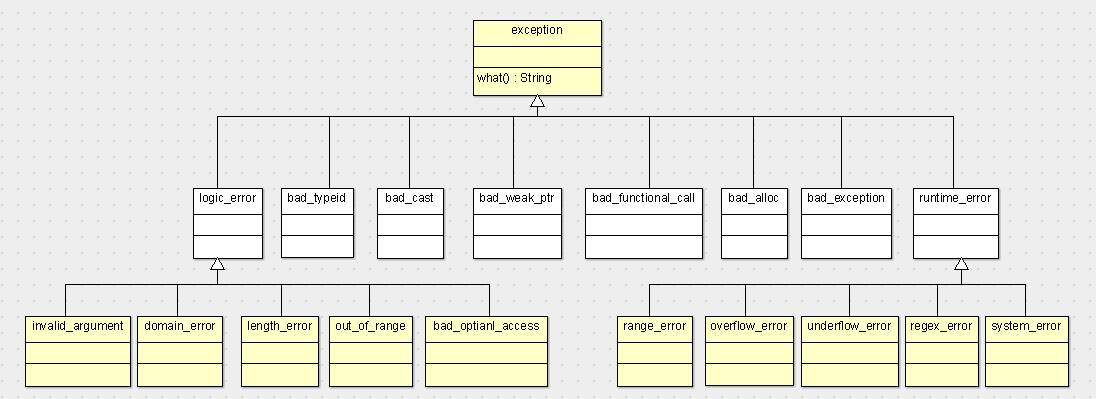
\includegraphics[scale = 0.45]{exception_level.png}
				\caption{Exception 层次结构}
			\end{figure}
		
		\subsection{C++ 异常机制的工作方式}
			当抛出异常时,其控制权 将转交给与其类型匹配的最近的处理代码
			
			运行时异常系统立即开始查找适合的catch块,此catch块必须与传递给throw 语句的参数相匹配。在过程内部,catch块必须在try 之后。
			
			当F()抛出一个异常时,异常从F()返回,并且不执行throw语句后的任何语句。 控制权返回给F()的调用者,即main()函数。 这种从F() 返回异常 与常规返回并无区别。 
			
			由于异常要离开F()之前,会调用所有局部对象的析构函数。换言之,从F()正常返回需要进行清理工作,由于异常返回也必须完成这些清理工作。
			
			异常会进行传播,直至遇到匹配的处理代码。异常只能由catch块处理。考虑到匹配的需要,catch块总是在try 块之后。try 块是编译器查找catch块的线索。 也就是说,try 块创建了一个动态调用链。一旦进入catch块就会立即处理异常,当退出相应的catch块时,异常结束(异常状况不再存在)
			
			如果main()中没有匹配的catch块,异常就仍然没有得到处理,而且,一旦控制从F()返回main(), 将调用预定义的terminate()。 注意,在这种情况下,绝不会执行try 块后的代码。一旦F()抛出异常,使得控制权返回main(),我们就正处于异常处理模式。函数terminate() 将导致应用程序异常终止。(参考自:\textbf{C++面向对象高效编程})
			
			\subsubsection{流程}见图\ref{process_error}
\begin{lstlisting}
	#include <iostream>
	
	using namespace std;
	
	int main()
	{
		try{
			cout << "Before Throw" << endl;
			throw 1;
			cout << "After Throw In Try" << endl;
		}
		catch (int& i)
		{
			cout << "After Throw In Catch" << endl;
		}
		
		//如果没有匹配的catch块,就会调用teminate():如果没设置teminate就终止程序..就不会执行下面的语句了
		
		cout << "Main!" << endl;
		cin.get();
	}
\end{lstlisting}
			
			\begin{figure}[h]
				\centering
				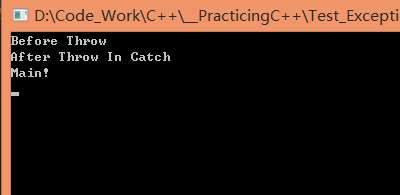
\includegraphics[scale = 1]{Exception_Process.png}
				\caption{流程演示}
				\label{process_error}
			\end{figure}
			
	\subparagraph{显示异常名字}
\begin{lstlisting}
	// 显示异常 的具体 代码
	#include <exception>
	#include <iostream>
	#include <cxxabi.h>
	
	struct empty { };
	
	template <typename T, int N>
	struct bar { };
	
	
	int main()
	{
		int     status;
		char   *realname;
		
		// exception classes not in <stdexcept>, thrown by the implementation
		// instead of the user
		std::bad_exception  e;
		realname = abi::__cxa_demangle(e.what(), 0, 0, &status);
		std::cout << e.what() << "\t=> " << realname << "\t: " << status << '\n';
		free(realname);
		
		
		// typeid
		bar<empty,17>          u;
		const std::type_info  &ti = typeid(u);
		
		realname = abi::__cxa_demangle(ti.name(), 0, 0, &status);
		std::cout << ti.name() << "\t=> " << realname << "\t: " << status << '\n';
		free(realname);
		
		return 0;
	}
	
	/*
	This prints 
	
	St13bad_exception       => std::bad_exception   : 0
	3barI5emptyLi17EE       => bar<empty, 17>       : 0
	*/
	
\end{lstlisting}	
		\subsection{其他}
			\subsubsection{std::variant}
				The class template std::variant represents\textbf{ a type-safe union}. An instance of std::variant at any given time either holds a value of one of its alternative types, or it holds no value (this state is hard to achieve, see valueless\_by\_exception).
				
				As with unions, if a variant holds a value of some object type T, the object representation of T is allocated directly within the object representation of the variant itself. Variant is not allowed to allocate additional (dynamic) memory.
				
				If a variant holds a value of a reference type, the implementation may choose to store it in the form of a wrapper type such as std::reference\_wrapper.
				
				A variant is permitted to hold the type void, to hold the same type more than once, and to hold differently cv-qualified versions of the same type.
				
				As with unions, the default-initialized variant holds a value of its first alternative, unless that alternative is not default-constructible (in which case default constructor won't compile: the helper class std::monostate can be used to make such variants default-constructible)
\begin{lstlisting}
	#include <variant>
	#include <string>
	
	int main()
	{
		std::variant<int, float> v, w;
		v = 12; // v contains int
		int i = std::get<int>(v);
		w = std::get<int>(v);
		w = std::get<0>(v); // same effect as the previous line
		w = v; // same effect as the previous line
		
		//  std::get<double>(v); // error: no double in [int, float]
		//  std::get<3>(v);      // error: valid index values are 0 and 1
		
		try {
			std::get<float>(w); // w contains int, not float: will throw
		}
		catch (std::bad_variant_access&) {}
		
		std::variant<std::string> v("abc"); // converting constructors work when unambiguous
		v = "def"; // converting assignment also works when unambiguous
	}
\end{lstlisting} 
	\section{logic\_error}
		Defines a type of object to be thrown as exception. It reports errors that are a consequence of faulty logic within the program such as violating logical preconditions or class invariants and \textbf{may be preventable.}
		\subsection{invalid\_argument}
			Defines a type of object to be thrown as exception. It reports errors that arise because an argument value has not been accepted.
			
			This exception is thrown by std::bitset::bitset, and the std::stoi and std::stof families of functions. 
		\subsection{domain\_error}
			Defines a type of object to be thrown as exception. It may be used by the implementation to report domain errors, that is, situations where the inputs are outside of the domain on which an operation is defined.
			
			The standard library components do not throw this exception (mathematical functions report domain errors as specified in math\_errhandling). Third-party libraries, however, use this. For example, boost.math throws std::domain\_error if boost::math::policies::throw\_on\_error is enabled (the default setting). 
		\subsection{length\_error}
			Defines a type of object to be thrown as exception. It reports errors that are consequence of attempt to exceed implementation defined length limits for some object.
			
			This exception is thrown by member functions of std::basic\_string and std::vector::reserve 
		\subsection{out\_of\_range}
			Defines a type of object to be thrown as exception. It reports errors that are consequence of attempt to access elements out of defined range.
			
			It may be thrown by the member functions of std::bitset and std::basic\_string, by std::stoi and std::stod families of functions, and by the bounds-checked member access functions (e.g. std::vector::at and std::map::at) 
		\subsection{future\_error}
			The class std::future\_error defines an exception object that is thrown on failure by the functions in the thread library that deal with asynchronous execution and shared states (std::future, std::promise, etc). Similar to std::system\_error, this exception carries an error code compatible with std::error\_code. 
		\subsection{bad\_optional\_access}
			Defines a type of object to be thrown by std::optional::value when accessing an optional object that does not contain a value. 
		
	\section{runtime\_error}
		\subsection{range\_error}
			Defines a type of object to be thrown as exception. It can be used to report range errors (that is, situations where a result of a computation cannot be represented by the destination type)
			
			The only standard library components that throw this exception are std::wstring\_convert::from\_bytes and std::wstring\_convert::to\_bytes.
			
			The mathematical functions in the standard library components do not throw this exception (mathematical functions report range errors as specified in math\_errhandling). 
		\subsection{overflow\_error}
			Defines a type of object to be thrown as exception. It can be used to report arithmetic overflow errors (that is, situations where a result of a computation is too large for the destination type)
			
			The only standard library components that throw this exception are std::bitset::to\_ulong and std::bitset::to\_ullong.
			
			The mathematical functions of the standard library components do not throw this exception (mathematical functions report overflow errors as specified in math\_errhandling). Third-party libraries, however, use this. For example, boost.math throws std::overflow\_error if boost::math::policies::throw\_on\_error is enabled (the default setting). 
		\subsection{underflow\_error}
			Defines a type of object to be thrown as exception. It may be used to report arithmetic underflow errors (that is, situations where the result of a computation is a subnormal floating-point value)
			
			The standard library components do not throw this exception (mathematical functions report underflow errors as specified in math\_errhandling). Third-party libraries, however, use this. For example, boost.math throws std::underflow\_error if boost::math::policies::throw\_on\_error is enabled (the default setting). 
		\subsection{regex\_error}
			Defines the type of exception object thrown to report errors in the regular expressions library. 
\begin{lstlisting}
	#include <regex>
	#include <iostream>
				
	int main()
	{
		try {
			std::regex re("[a-b][a");
		} 
					
		catch (const std::regex_error& e) {
			std::cout << "regex_error caught: " << e.what() << '\n';
			if (e.code() == std::regex_constants::error_brack) {
				std::cout << "The code was error_brack\n";
				}
		}
	}
\end{lstlisting}
		\subsection{system\_error}
			std::system\_error is the type of the exception thrown by various library functions (typically the functions that interface with the OS facilities, e.g. the constructor of std::thread) when the exception has an associated std::error\_code, which may be reported. 
			\subsubsection{ios\_base::failure}
				The class std::ios\_base::failure defines an exception object that is thrown on failure by the functions in the Input/Output library.
				
				std::ios\_base::failure may be defined either as a member class of std::ios\_base or as a synonym (typedef) for another class with equivalent functionality. 
				
\begin{lstlisting}
	#include <iostream>
	#include <fstream>
	int main()
	{
		std::ifstream f("doesn't exist");
		try {
			f.exceptions(f.failbit);
		} catch (const std::ios_base::failure& e)
		{
			std::cout << "Caught an ios_base::failure.\n"
			<< "Explanatory string: " << e.what() << '\n'
			<< "Error code: " << e.code() << '\n';
		}
	}
					
	/*
		Caught an ios_base::failure.
		Explanatory string: ios_base::clear: unspecified iostream_category error
		Error code: iostream:1
	*/
				\end{lstlisting}
			\subsubsection{filesystem::filesystem\_error}
				The class std::filesystem::filesystem\_error defines an exception object that is thrown on failure by the throwing overloads of the functions in the filesystem library. 
				
		\subsection{tx\_exception}
				Defines an exception type that can be used to cancel and roll back an atomic transaction initiated by the keyword atomic\_cancel
					
				If T is not TriviallyCopyable, the program that specializes std::tx\_exception<T> is ill-formed. 
	\section{bad errors}
		\subsection{bad\_typeid}
			An exception of this type is thrown when a typeid operator is applied to a dereferenced null pointer value of a polymorphic type.
			
\begin{lstlisting}
	#include <iostream>
	#include <typeinfo>
	
	struct S { // The type has to be polymorphic
		virtual void f();
	}; 
	
	int main()
	{
		S* p = nullptr;
		try {
			std::cout << typeid(*p).name() << '\n';
		} catch(const std::bad_typeid& e) {
		std::cout << e.what() << '\n';
		}
	}
	
	//Attempted a typeid of NULL pointer!
\end{lstlisting}
		\subsection{bad\_cast}
			\subsubsection{bad\_any\_cast}
				Defines a type of object to be thrown by the value-returning forms of std::any\_cast on failure. 
		\subsection{bad\_weak\_ptr}
			std::bad\_weak\_ptr is the type of the object thrown as exceptions by the constructors of std::shared\_ptr that take std::weak\_ptr as the argument, when the std::weak\_ptr refers to an already deleted object. 
\begin{lstlisting}
	#include <memory>
	#include <iostream>
	int main()
	{
		std::shared_ptr<int> p1(new int(42));
		std::weak_ptr<int> wp(p1);
		p1.reset();
		try {
			std::shared_ptr<int> p2(wp);
		} catch(const std::bad_weak_ptr& e) {
			std::cout << e.what() << '\n';
		}
	}
	
	//std::bad_weak_ptr
\end{lstlisting}
		\subsection{bad\_function\_call}
			std::bad\_function\_call is the type of the exception thrown by std::function::operator() if the function wrapper has no target. 
\begin{lstlisting}
	#include <iostream>
	#include <functional>
	
	int main()
	{
		std::function<int()> f = nullptr;
		try {
			f();
		} catch(const std::bad_function_call& e) {
			std::cout << e.what() << '\n';
		}
	}
	
	//bad function call
\end{lstlisting}
		\subsection{bad\_alloc}
			std::bad\_alloc is the type of the object thrown as exceptions by the allocation functions to report failure to allocate storage
\begin{lstlisting}
	#include <iostream>
	#include <new>
	
	int main()
	{
		try {
				while (true) {
					new int[100000000ul];
				}
			} catch (const std::bad_alloc& e) {
			std::cout << "Allocation failed: " << e.what() << '\n';
		}
	}
	
	//Allocation failed: std::bad_alloc
\end{lstlisting}
		\subsection{bad\_exception}
			std::bad\_exception is the type of the exception thrown by the C++ runtime in the following situations: 
			
			\begin{enumerate}
				\item If a dynamic exception specification is violated and std::unexpected throws or rethrows an exception that still violates the exception specification, but the exception specification allows std::bad\_exception, std::bad\_exception is thrown.
				\item If std::exception\_ptr stores a copy of the caught exception and if the copy constructor of the exception object caught by current\_exception throws an exception, the captured exception is an instance of std::bad\_exception.
			\end{enumerate}

\begin{lstlisting}
	#include <iostream>
	#include <exception>
	#include <stdexcept>
	
	void my_unexp() { throw; }
	
	void test() throw(std::bad_exception)
	{
		throw std::runtime_error("test");
	}
	
	int main()
	{
		std::set_unexpected(my_unexp);
		try {
			test();
		} catch(const std::bad_exception& e)
		{
			std::cerr << "Caught " << e.what() << '\n';
		}
	}
	
	//Caught std::bad_exception
\end{lstlisting}
		\subsection{bad\_variant\_access}
			std::bad\_variant\_access is the type of the exception thrown in the following situations: 
			\begin{itemize}
				\item std::get(std::variant) called with an index or type that does not match the currently active alternative 
				\item  std::visit called to visit a variant that is valueless\_by\_exception 
			\end{itemize}
\begin{lstlisting}
	#include <variant>
	#include <iostream>
	
	int main()
	{
		std::variant<int, float> v;
		v = 12;
		try {
			std::get<float>(v);
		}
		catch(const std::bad_variant_access& e) {
			std::cout << e.what() << '\n';
		}
	}
	
	//bad_variant_access
\end{lstlisting}

%%%%%%%%%%%%%%%%%%%%%%%%%%%%%%%%%%%%%%%%%%%%%%%%%%%%%%%%%%%%%%%%%%%%%%%CHAPTER_MULTITRHEAD%%%%%%%%%%%%%%%%%%%%%%%%%%%%%%%%%%%%%%%%%%%%%%%%%%%%%%%%%%%%%%%%%%%%%%%%%%
\chapter{多线程}
\section{参考}
	多线程使用:\url{http://www.tuicool.com/articles/VFjyYnq}
		
		\url{http://www.2cto.com/kf/201507/419768.html}
		
		\url{http://www.2cto.com/kf/201504/390787.html}
		
		\url{http://blog.jobbole.com/81265/}
	
	内部实现源码:\url{http://blog.jobbole.com/105900/}
	
\section{须知}
	\subsection{线程安全}
		\textbf{线程安全}就是多线程访问时,采用了加锁机制,当一个线程访问该类的某个数据时,进行保护,其他线程不能进行访问直到该线程读取完,其他线程才可使用。不会出现数据不一致或者数据污染。 线程不安全就是不提供数据访问保护,有可能出现多个线程先后更改数据造成所得到的数据是脏数据
		
		比如一个 ArrayList 类,在添加一个元素的时候,它可能会有两步来完成:1. 在 Items[Size] 的位置存放此元素;2. 增大 Size 的值。
		
		在单线程运行的情况下,如果 Size = 0,添加一个元素后,此元素在位置 0,而且 Size=1;
		
		而如果是在多线程情况下,比如有两个线程,线程 A 先将元素1存放在位置 0。但是此时 CPU 调度线程A暂停,线程 B 得到运行的机会。线程B向此 ArrayList 添加元素2,因为此时 Size 仍然等于 0 (注意,我们假设的是添加一个元素是要两个步骤,而线程A仅仅完成了步骤1),所以线程B也将元素存放在位置0。然后线程A和线程B都继续运行,都增加 Size 的值,结果Size等于2。
		那好,我们来看看 ArrayList 的情况,期望的元素应该有2个,而实际只有一个元素,造成丢失元素,而且Size 等于 2。这就是“线程不安全”了
		\subparagraph{线程安全的条件}
			\begin{itemize}
				\item 多个线程同时访问时,其表现出正确的行为。
				\item 无论操作系统怎么调度这些线程,无论这些线程的执行顺序如何交织
				\item 调用端代码 \textbf{无须额外的同步}或其他协调动作。
			\end{itemize}
		\subparagraph{线程安全的类}可以通过 同步原语(类自身拥有的mutex(互斥器)来) 保护内部状态。
		\subparagraph{对象的race condition}这个不能由类自身拥有的mutex(互斥器)来保护,可以借助boost 的shared,weaked ptr 实现的observer 模式解决。
		
		\subsection{对象的创建}
			对象构造时要\textbf{做到}\underline{线程安全},唯一要求是在构造期间不要泄露this指针,即:
				\begin{itemize}
					\item 不要在构造函数中注册任何回调
					\item 不要在构造函数中将this传给跨线程的对象
					\item 即便在最后一行也不行:派生会先执行父类的构造的,而你写的可能就是父类..这样对方就讲返回一个半成品..
				\end{itemize}
		
\section{使用}
	\subsection{头文件}
		\begin{itemize}
			\item \textbf{<atomic>}: 包含std::atomic和std::atomic\_flag类,以及一套C风格的原子类型和与C兼容的原子操作的函数。
			\item \textbf{<thread>}: 包含std::thread类以及std::this\_thread命名空间。
			\item \textbf{<mutex>}: 包含与互斥量(mutex)相关的类以及其他类型和函数。
			\item \textbf{<condition\_variable>}: 包含与条件变量相关的类, 包括std::condition\_variable 和
			
			 std::condition\_variable\_any。
			\item \textbf{<future>}:包含两个Provider类(std::promise和std::package\_task)和两个Future类(std::future和std::shared\_future)以及相关的类型和函数
		\end{itemize}
		
	\subsection{多线程}
		C++11中使用多线程非常简单,直接使用头文件thread中的thread类型即可创建一个线程,具体例子如下所示:
		\begin{lstlisting}
	#include <iostream>
	#include <thread>
	#include <string>
	using namespace std;
	
	void Func();
	
	int main()
	{
		//线程函数无参数- 使用Lamda 进行函数设置..
		thread t([](){ cout << "Hello World!" << endl; });
		//当然也可以 直接以指定函数的方式初始化 线程
		thread t1(Func);
		t.join(); //t1线程调用t2.join(),表示t1要等到t2结束后才能继续执行
	}
		\end{lstlisting}
		
		这里涉及到多线程环境中父子线程的关系问题。一般操作系统中,\textbf{当主线程执行完毕退出时,无论子线程是否执行完毕,所有的子线程都会终止}。\textbf{而当子线程先退出时,无论是执行完毕正常退出还是以其他方式异常终止,线程均会进入终止态(僵死态),此时线程分配的系统资源还没有释放},线程仍作为一个线程实体存在于操作系统中。\textbf{如果我们就这样不管这个子线程,那么它占用的系统资源(如动态申请的内存、打开的文件等)将一直被占据,造成资源的浪费}。此时可以通过定义以下两种父子线程关系进行解决:
		
		\begin{itemize}
			\item \textbf{可会和}(joinable):主线程必须显示等待子线程,只有子线程结束后,主线程才继续执行后面的操作
			\item \textbf{相分离}(detached):父子线程分离,主线程无须等待子线程完成,子线程一旦进入终止态后系统立即销毁线程以及回收资源
		\end{itemize}
		
		\subparagraph{Funcs:}thread头文件的\textbf{this\_thread命名空间}定义了几个有用的函数:
		\begin{itemize}
			\item \textbf{get\_id}:    返回当前的线程id
			\item \textbf{yield}:  	   在处于等待状态时,可以让调度器先运行其他可用的线程
			\item \textbf{sleep\_for}: 阻塞当前线程,时间不少于参数指定的时间
			\item \textbf{sleep\_util}:阻塞当前线程,时间为参数指定的时间
		\end{itemize}
		\begin{lstlisting}
	#include <iostream>
	#include <thread>
	#include <string>
	using namespace std;
	
	void f()
	{
		// Using ID to Distinguishing threads 
		cout << "Thread ID: " << this_thread::get_id() << endl;
		this_thread::sleep_for(chrono::seconds(3));
	}
	
	int main()
	{
		thread t1(f);
		//输出线程id和cpu核数
		std::cout << ID: << t1.get_id() << std::endl;
		std::cout << CPU: << std::thread::hardware_concurrency() << std::endl;
		//主函数阻塞等待线程结束
		t1.join();
		//主函数和线程函数分离执行,线程变为后台线程,与t1.join() 互斥
		//t1.detach();
	}
		\end{lstlisting}
		\subsection{初始化线程}
		首先其类模板模型如下图所示:
		\begin{figure}[h]
			\centering
			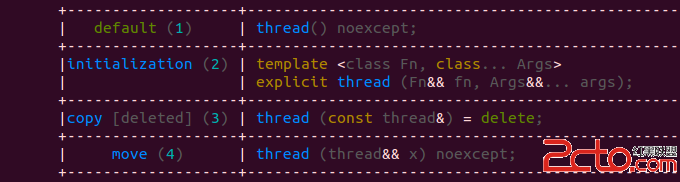
\includegraphics[scale= 0.8]{thread.png}
			\caption{Thread Pattern}
		\end{figure}
		\begin{lstlisting}
	namespace std
	{
		struct thread
		{
			// native_handle_type 是连接 thread 类和操作系统 SDK API 之间的桥梁。
			typedef implementation-dependent native_handle_type;
			native_handle_type native_handle();
			// 线程ID
			struct id
			{
				id() noexcept;
				// 可以由==, < 两个运算衍生出其它大小关系运算。
				bool operator==(thread::id x, thread::id y) noexcept;
				bool operator<(thread::id x, thread::id y) noexcept;
				template<class charT, class traits>
				basic_ostream<charT, traits>&
				operator<<(basic_ostream<charT, traits>&out, thread::id id);
				// 哈希函数
				template <class T> struct hash;
				template <> struct hash<thread::id>;
			};
			id get_id() const noexcept;
			// 构造与析构
			thread() noexcept;
			// 注意:前面为函数,后面为函数的参数表..的实参值.
			template<class F, class… Args> explicit thread(F&f, Args&&… args);
			~thread();
			thread(const thread&) = delete;
			thread(thread&&) noexcept;
			thread& operator=( const thread&) = delete;
			thread& operator=(thread&&) noexcept;
			//
			void swap(thread&) noexcept;
			bool joinable() const noexcept;
			void join();
			void detach();
			// 获取物理线程数目
			static unsigned hardware_concurrency() noexcept;
		}
		
		namespace this_thead
		{
			thread::id get_id();
			void yield();
			template<class Clock, class Duration>
			void sleep_until(const chrono::time_point<Clock, Duration>& abs_time);
			template<class Rep, class Period>
			void sleep_for(const chromo::duration<Rep, Period>& rel_time);
		}
	}	
		\end{lstlisting}
		
		\subparagraph{初始化方式..}
		\begin{enumerate}[itemindent = 1em]
			\item \textbf{thread\_run\_func\_var\_args}:
			\begin{lstlisting}
	#include <iostream>
	#include <thread>
			
	using namespace std;
			
	void myFirstThreadTask(int num)
	{
		for (int i = 0; i < 10; ++i)
		{
			cout << "myFirstThreadTask's num = " << num++ << endl;
			this_thread::sleep_for(chrono::milliseconds(10));
		}
	}
			
	void mySecondThreadTask(int &num)
	{
		for (int i = 0; i < 10; ++i)
		{
			cout << "mySecondThreadTask's num = " << num++ << endl;
			this_thread::sleep_for(std::chrono::milliseconds(10));
		}
	}
			
	int _tmain(int argc, _TCHAR* argv[])
	{
		int n = 5;
		thread myThread0;//myThread1为一个空线程,不代表任何可执行对象
			
		//myThread1与myFirstThreadTask函数绑定,n为其按值传递参数
		thread myThread1(myFirstThreadTask,n);
			
		//myThread2与mySecondThreadTask函数绑定,n为其引用传递参数
		thread myThread2(mySecondThreadTask,std::ref(n));
		myThread1.join();
		myThread2.join();
			
		n++;
			
		//现在myThread2不代表任何可执行对象,myThread3与mySecondThreadTask函数绑定
		thread myThread3(std::move(myThread2));
		//myThread3.join();
		return 0;
	}
			\end{lstlisting}
			\item \textbf{thread\_run\_lambda}:
			\begin{lstlisting}
	void threadRunLambda(void)
	{
		int a = 100,
		b = 200;
		thread* t = new thread( 
		[](int ia, int ib)
		{
		cout << (ia + ib) << endl;
		},
		a,
		b );
			
		t->join();
		delete t;
	}
			\end{lstlisting}
			\item \textbf{thread\_run\_member\_func}:
			\begin{lstlisting}
// Method1:
	struct God
	{
		void create(string& anything)
		{
			cout << "create " << anything << endl;
		}
	};
			
	void threadRunMemberFunction(void)
	{
		God god;
		string s = "some";
		thread* t = new thread( &God::create, god, s );// 虽然函数定义为引用,但是还是值传递参数,如果需要引用,需要添加std::ref(s);
		// t = new thread(&God::create,god,std::ref(s)); 这样才会真正的引用传递参数
		t->join();
		delete t;
	}

// Method2:
	class Factor{
	public:
		void operater() (){
			cout <<"create"<<endl;
		}
	};

	void threadRunObject(void)
	{
		Factor factor;
		thread t(factor);
		t.join();
	}
			\end{lstlisting}
		\end{enumerate}
		
		\subsection{线程间数据交互和数据争用(Data Racing)}
		同一个进程内的多个线程之间多是免不了要有数据互相来往的,队列和共享数据是实现多个线程之间的数据交互的常用方式,封装好的队列使用起来相对来说不容易出错一些,而共享数据则是最基本的也是较容易出错的,因为它会产生数据争用的情况,即有超过一个线程试图同时抢占某个资源,比如对某块内存进行读写等,如下例所示:
		\begin{lstlisting}
static void inc(int *p)
{
	for(int i = 0; i < COUNT; ++i)
	(*p)++;
}
		
void ThreadDataRacing()
{
	int a = 0;
	thread th1(inc, &a);
	thread th2(inc, &a);
		
	th1.join();
	th2.join();
		
	cout<<"a = "<<a<<endl;
}
		\end{lstlisting}
		
		这是简化了的极端情况,我们可以一眼看出来这是两个线程在同时对\&a 这个内存地址进行写操作,但是在实际工作中,在代码的海洋中发现它并不一定容易。从表面看,两个线程执行完之后,最后的 a 值应该是 COUNT * 2,但是实际上并非如此,\textbf{因为简单如 (*p)++这样的操作并不是一个原子动作,要解决这个问题,对于简单的基本类型数据如字符、整型、指针等,C++提供了原子模版类 atomic},\underline{而对于复杂的对象},\textbf{则提供了最常用的锁机制,比如互斥类 mutex,门锁 lock\_guard,唯一锁 unique\_lock,条件变量 condition\_variable 等}。
		
		\subparagraph{解决方案:}
		\begin{enumerate}[itemindent = 1em]
			\item \textbf{atomic}:针对简单的基本类型数据如字符、整型、指针等
			\begin{lstlisting}
static void inc(atomic<int> *p )
{
	for(int i = 0; i < COUNT; i++)
	{
		(*p)++;
	}
}
void threadDataRacing(void)
{
	atomic<int> a(0) ;
				
	thread ta( inc, &a);
	thread tb( inc, &a);
				
	ta.join();
	tb.join();
				
	cout << "a=" << a << endl;
}
			\end{lstlisting}
			\item \textbf{lock\_guard}:lock\_guard 是一个\textbf{范围锁},本质是 RAII(Resource Acquire Is Initialization),在构建的时候自动加锁,在析构的时候自动解锁,这保证了每一次加锁都会得到解锁。即使是调用函数发生了异常,在清理栈帧的时候也会调用它的析构函数得到解锁,从而保证每次加锁都会解锁,但是我们不能手工调用加锁方法或者解锁方法来进行更加精细的资源占用管理
			\begin{lstlisting}
static mutex g_mutex;
static void inc(int *p )
{
	for(int i = 0; i < COUNT; i++)
	{
	lock_guard<mutex> _(g_mutex);
		(*p)++;
	}
}
			
void threadLockGuard(void)
{
	int a = 0;
			
	thread ta( inc, &a);
	thread tb( inc, &a);
			
	ta.join();
	tb.join();
			
	cout << "a=" << a << endl;
}
			\end{lstlisting}
			\item \textbf{mutex}:如果要\textbf{支持手工加锁},可以考虑使用 unique\_lock 或者直接使用 mutex。unique\_lock 也支持 RAII,它也可以一次性将多个锁加锁;如果使用 mutex 则直接调用 mutex 类的 lock, unlock, trylock 等方法进行更加精细的锁管理
			
			Mutual exclusion algorithms \textbf{prevent} multiple threads from simultaneously accessing shared resources. This prevents data races and provides support for synchronization between threads.
			\begin{lstlisting}
static mutex g_mutex;
static void inc(int *p )
{
	thread_local int i; // TLS 变量
	for(; i < COUNT; i++)
	{
		g_mutex.lock();
		(*p)++;
		g_mutex.unlock();
	}
}
			
void threadMutex(void)
{
	int a = 0;
			
	thread ta( inc, &a);
	thread tb( inc, &a);
			
	ta.join();
	tb.join();
	cout << "a=" << a << endl;
}
			\end{lstlisting}
			\item \textbf{conditon\_variable}:在上例中,我们还使用了线程本地存储 (TLS) 变量,我们只需要在变量前面声明它是 thread\_local 即可。TLS 变量在线程栈内分配,线程栈只有在线程创建之后才生效,在线程退出的时候销毁,需要注意不同系统的线程栈的大小是不同的,如果 TLS 变量占用空间比较大,需要注意这个问题。TLS 变量一般不能跨线程,其初始化在调用线程第一次使用这个变量时进行,默认初始化为 0。
			
			A condition variable is a synchronization primitive that allows multiple threads to communicate with each other. It allows some number of threads to wait (possibly with a timeout) for notification from another thread that they may proceed. A condition variable is always associated with a mutex.
			
			对于线程间的事件通知,C++11 提供了条件变量类 condition\_variable,可视为 pthread\_cond\_t 的封装,使用条件变量可以让一个线程等待其它线程的通知 (wait,wait\_for,wait\_until),也可以给其它线程发送通知 (notify\_one,notify\_all),条件变量必须和锁配合使用,在等待时因为有解锁和重新加锁,所以,在等待时必须使用可以手工解锁和加锁的锁,比如 unique\_lock,而不能使用 lock\_guard
			\begin{lstlisting}
#include <condition_variable>
mutex m;
condition_variable cv;
void threadCondVar(void)
{
	# define THREAD_COUNT 10
	thread** t = new thread*[THREAD_COUNT];
	int i;
	for(i = 0; i < THREAD_COUNT; i++)
	{
		t[i] = new thread( [](int index){
			unique_lock<mutex> lck(m);
			cv.wait_for(lck, chrono::hours(1000));
			cout << index << endl;
			}, i );
			
		this_thread::sleep_for( chrono::milliseconds(50));
	}
	for(i = 0; i < THREAD_COUNT; i++)
	{
		lock_guard<mutex> _(m);
		cv.notify_one();
	}
	for(i = 0; i < THREAD_COUNT; i++)
	{
		t[i]->join();
		delete t[i];
	}
	delete t;
}
			\end{lstlisting}
		\end{enumerate}
	\subsection{互斥锁}
		多线程编程一般避免不了同步的问题,C++11这里也提供了非常方便的方法来进行解决。标准中提供了一下四种互斥锁,分别是:
		\begin{itemize}
			\item  \textbf{Mutex}:基本的Mutex类,\textbf{独占的互斥量,不能递归使用},提供了核心函数lock()和unlock()
			\item  \textbf{Recursive\_mutex}:递归Mutex类,\textbf{递归互斥量,不带超时功能},允许在同一个线程中对一个互斥量的多次请求。一般在项目模块分工中可以使用,这样即使其他人使用了同样的锁也不会导致死锁
			\item \textbf{Timed\_mutex}:定时递归Mutex类,\textbf{带超时的独占的互斥量,不能递归使用},除了递归,还可以在某个时间段里或者某个时刻到达之间获取该互斥量。当一个线程在临界区操作的时间非常长,可以用定时锁指定时间
			\item \textbf{Recursive\_timed\_mutex}:定时递归Mutex类,\textbf{带超时的递归互斥量},综合timed\_mutex和recuseive\_mutex
		\end{itemize}
		
		下面是一个使用基本锁的小例子,该程序会按顺序输出5对enter和leave,分别对应5个线程。如果注释掉函数f中mt的lock和unlock函数,则线程没有同步,此时先输出5句enter,然后5s后再输出5句leave.
		\subsubsection{Mutex}
			\begin{lstlisting}
	#include <iostream>
	#include <thread>
	#include <string>
	#include <mutex>
	#include <vector>
	using namespace std;
	
	mutex mt; //注意,全局的哟..
	
	void f()
	{
		mt.lock();
		cout << "Enter Critical Section" << endl;
		this_thread::sleep_for(chrono::seconds(5));
		cout << "Leave Critical Section" << endl;
		mt.unlock();
	}
	
	int main()
	{
		vector<thread> v(5);
		for (auto &i : v) i = thread(f);
		for (auto &i : v) i.join();
	}
		\end{lstlisting}
		\subparagraph{lock\_guard<T\_mutex> m(T\_mutex)}:从对象初始化时 到 对象销毁时
		
		\subparagraph{unique\_lock<T\_mutex> m(T\_mutex)}:提供比lock\_guard 更灵活的方式,可以指定什么时候上锁,什么时候解锁,但是可以保证任何时候都会在析构时将锁释放掉。
			\begin{lstlisting}
void func()
{
	// 当作用域为函数的全部作用域时,lock_guard 与 unique_lock 起到了同样的作用
	lock_guard<std::mutex>locker(mutex);
	unique_lock<std::mutex>locker2(mutex2);
	
	// 但是在申请锁的时候不想上锁,lock_guard 就不行了,这是unique_lock 可以这样做
	unique_lock<std::mutex>locker3(mutex3, std::defer_lock);
		...stuff
		locker3.lock();
		...stuff..
		// 在处理玩这些事之后 就不需要锁了,unique 可以unlock()
		locker3.unlock();
		...stuff
		// 又需要了
		locker3.lock();
		
		// 而且unique_lock 可以被移动,而lock_guard 不可以,但是两者都不可以复制	
		unique_lock<std::mutex> locker4 = std::move(locker3);	
}	
			\end{lstlisting}
		\subparagraph{Recursice\_mutex}
			为什么需要使用 Recursive\_mutex,看例子
			\begin{lstlisting}
struct Complex {
	std::mutex mutex;
	int i;
	
	Complex() : i(0) {}
	
	void mul(int x){
		std::lock_guard<std::mutex> lock(mutex);
		i *= x;
	}
	
	void div(int x){
		std::lock_guard<std::mutex> lock(mutex);
		i /= x;
	}
	
	void both(int x, int y){
		std::lock_guard<std::mutex> lock(mutex);
		mul(x);
		div(y);
	}
};	
	
int main(){
	Complex complex;
	complex.both(32, 23);
	
	return 0;
}

//If you launch this application, you'll see that the program will never terminates. The problem is very simple. In the both() function, the thread acquires the lock and then calls the mul() function. In this function, the threads tries to acquire the lock again, but the lock is already locked. This is a case of deadlock. By default, a thread cannot acquire the same mutex twice.
			\end{lstlisting}
		
			\textbf{There is a simple solution to this problem: std::recursive\_mutex}. This mutex can be acquired several times by the same thread.
			\begin{lstlisting}
struct Complex {
	std::recursive_mutex mutex;
	int i;
	
	Complex() : i(0) {}
	
	void mul(int x){
		std::lock_guard<std::recursive_mutex> lock(mutex);
		i *= x;
	}
	
	void div(int x){
		std::lock_guard<std::recursive_mutex> lock(mutex);
		i /= x;
	}
	
	void both(int x, int y){
		std::lock_guard<std::recursive_mutex> lock(mutex);
		mul(x);
		div(y);
	}
};	

//This time, the application works correctly.		
			\end{lstlisting}
	\subsubsection{Call once}
		Sometimes \textbf{you want a function to be called only once no matter the number of threads that are used}. Imagine a function that has two parts. The first part has to be called only once and the second has to be executed every time the function gets called. We can use the std::call\_once function to fix this problem very easily.
		
		\begin{lstlisting}
std::once_flag flag;

void do_something(){
	std::call_once(flag, [](){std::cout << "Called once" << std::endl;});
	
	std::cout << "Called each time" << std::endl;
}

int main(){
	std::thread t1(do_something);
	std::thread t2(do_something);
	std::thread t3(do_something);
	std::thread t4(do_something);
	
	t1.join();
	t2.join();
	t3.join();
	t4.join();
	
	return 0;
}			
		\end{lstlisting}
	\subparagraph{注意:}
		\begin{enumerate}[itemindent = 1em]
			\item 多次获取互斥量可能会发生死锁,所以我们调用std::recursive\_mutex递归锁,允许同一线程多次获得该锁,\textbf{一般不要使用递归锁},原因:
				\begin{itemize}
					\item 用到递归锁会使得程序的逻辑变复杂,使用到递归锁的程序一般可以简化
					\item 递归锁比非递归锁效率低
					\item 递归锁的可重入次数是有限的,超过也会报错
				\end{itemize}
			\item 可以使用带超时时间的互斥锁,避免阻塞在等待互斥锁上
			\item unique\_lock: 是一个通用的互斥量封装类。与lock\_guard不同,它还支持延迟加锁、时间锁、递归锁、锁所有权的转移并且还支持使用条件变量。这也是一个不可复制的类,但它是可以移动的类
		\end{enumerate}
		
		Keep in mind that \textbf{locks are slow}. Indeed, when you use locks you make sections of the code sequential. \textbf{If you want an highly parallel application}, there are other solutions than locks that are performing much better.
	\subsection{条件变量}
		条件变量condition\_variable\textit{也可以}\textbf{进行线程之间的通信},\textit{当一个线程要等待另一个线程完成某个操作时},\textbf{可以使用条件变量进行实现}。\textit{条件变量可以将一个或多个线程进入阻塞状态,直到收到另外一个线程的通知,或者超时才能退出阻塞状态}。
		
		\textbf{一个线程等待某个条件满足},其首先获得一个unique\_lock锁。该锁将会传递给wait()方法,然后wait()方法会释放互斥量并将该线程暂停,\textbf{直到条件变量得到相应的信号}。当接受到信号,线程被唤醒后,该锁就又被重新获得了。
		
		\textbf{另外一个线程发送信号使得条件满足}。其通过调用notify\_one()来发送通知,会将处于阻塞状态的等待该条件获得信号的线程中的某一个线程(\textbf{任意一个线程)恢复执行};还可以通过调用notify\_all()将\textbf{等待该条件的所有线程唤醒}。
		
		下面是一个使用条件变量的简单例子。该程序中f1等待某个条件,该条件在f2输出并且睡眠2s后才得到满足,之后f1才能够进行输出:

		\begin{lstlisting}
//A condition variable manages a list of threads waiting until another thread notify them. Each thread that wants to wait on the condition variable has to acquire a lock first. The lock is then released when the thread starts to wait on the condition and the lock is acquired again when the thread is awakened.

//A very good example is a concurrent Bounded Buffer. It’s a cyclic buffer with a certain capacity with a start and an end. Here is our implementation of a Bounded Buffer using condition variables:
#include <mutex>
#include <condition_variable>
#include <thread>
#include <iostream>

using namespace std;

struct BoundedBuffer {
	int* buffer;
	int capacity;
	
	int front;
	int rear;
	int count;
	
	std::mutex lock;
	
	std::condition_variable not_full;
	std::condition_variable not_empty;
	
	BoundedBuffer(int capacity) : capacity(capacity), front(0), rear(0), count(0) {
		buffer = new int[capacity];
	}

~BoundedBuffer(){
		delete[] buffer;
	}

void deposit(int data){
		std::unique_lock<std::mutex> l(lock);
		
		not_full.wait(l, [this](){return count != capacity; });
		
		buffer[rear] = data;
		rear = (rear + 1) % capacity;
		++count;
		
		not_empty.notify_one();
	}

int fetch(){
		std::unique_lock<std::mutex> l(lock);
		
		not_empty.wait(l, [this](){return count != 0; });
		
		int result = buffer[front];
		front = (front + 1) % capacity;
		--count;
		
		not_full.notify_one();
		
		return result;
	}
};

void consumer(int id, BoundedBuffer& buffer){
	for (int i = 0; i < 50; ++i){
		int value = buffer.fetch();
		std::cout << "Consumer " << id << " fetched " << value << std::endl;
		std::this_thread::sleep_for(std::chrono::milliseconds(250));
	}
}

void producer(int id, BoundedBuffer& buffer){
	for (int i = 0; i < 75; ++i){
		buffer.deposit(i);
		std::cout << "Produced " << id << " produced " << i << std::endl;
		std::this_thread::sleep_for(std::chrono::milliseconds(100));
	}
}

int main(){
	BoundedBuffer buffer(200);
	
	std::thread c1(consumer, 0, std::ref(buffer));
	std::thread c2(consumer, 1, std::ref(buffer));
	std::thread c3(consumer, 2, std::ref(buffer));
	std::thread p1(producer, 0, std::ref(buffer));
	std::thread p2(producer, 1, std::ref(buffer));
	
	c1.join();
	c2.join();
	c3.join();
	p1.join();
	p2.join();
	
	return 0;
}
		\end{lstlisting}
	\subsection{异步操作-async}
		C++11中的future是标准库提供的一种\textbf{用于获取异步操作的结果的机制},\textit{其可以调用一个函数,然后转而做其他的事情,让函数自己在一边执行,当需要的时候再回过头来获取该函数计算的结果}。另外,其还可以延迟异步操作中异常(Exception)的抛出。下面是一个简单的例子
		
		\subsubsection{future}
			std::future 可以用来\textbf{获取异步任务的结果},因此可以把它当成一种简单的线程间同步的手段。\textit{std::future 通常}\textbf{由某个 Provider 创建},你可以把 Provider 想象成一个异步任务的提供者,\textbf{Provider 在某个线程中设置共享状态的值},\textbf{与该共享状态相关联的 std::future 对象调用 get(通常在另外一个线程中) 获取该值},\textit{如果共享状态的标志不为 ready,则调用 std::future::get 会阻塞当前的调用者,直到 Provider 设置了共享状态的值(此时共享状态的标志变为 ready)},std::future::get 返回异步任务的值或异常(如果发生了异常)。
			
			一个有效(valid)的 std::future 对象通常由以下三种 Provider 创建,并和某个共享状态相关联。Provider 可以是函数或者类,其实我们前面都已经提到了,他们分别是:
				\begin{itemize}
					\item \textbf{std::async} 函数
					\item \textbf{std::promise::get\_future},get\_future 为 promise 类的成员函数
					\item \textbf{std::packaged\_task::get\_future},此时 get\_future为 packaged\_task 的成员函数
				\end{itemize}

			一个 std::future 对象只有在有效(valid)的情况下才有用(useful),由 std::future 默认构造函数创建的 future 对象不是有效的(除非当前非有效的 future 对象被 move 赋值另一个有效的 future 对象)。
			
			在一个有效的 future 对象上调用 get 会阻塞当前的调用者,直到 Provider 设置了共享状态的值或异常(此时共享状态的标志变为 ready),std::future::get 将返回异步任务的值或异常(如果发生了异常)。
\begin{lstlisting}
#include <iostream>       // std::cout
#include <future>         // std::async, std::future
#include <chrono>         // std::chrono::milliseconds

// a non-optimized way of checking for prime numbers:
bool is_prime (int x) {
	for (int i=2; i<x; ++i) if (x%i==0) return false;
	return true;
}

int main ()
{
	// call function asynchronously:
	std::future<bool> fut = std::async (is_prime,444444443); 
	
	// do something while waiting for function to set future:
	std::cout << "checking, please wait";
	std::chrono::milliseconds span (100);
	while (fut.wait_for(span)==std::future_status::timeout)
	std::cout << '.' << std::flush;
	
	bool x = fut.get();     // retrieve return value
	
	std::cout << "\n444444443 " << (x?"is":"is not") << " prime.\n";
	
	return 0;
}

//checking, please wait........................
//444444443 is prime.
\end{lstlisting}
		\subsubsection{promise}
			promise 对象可以保存某一类型 T 的值,该值可被 future 对象读取(可能在另外一个线程中),因此 promise 也提供了一种线程同步的手段。在 promise 对象构造时可以和一个共享状态(通常是std::future)相关联,并可以在相关联的共享状态(std::future)上保存一个类型为 T 的值。
			
			可以通过 get\_future 来获取与该 promise 对象相关联的 future 对象,调用该函数之后,两个对象共享相同的共享状态(shared state)
				\begin{itemize}
					\item \textbf{promise} 对象是异步 Provider,它可以在某一时刻设置共享状态的值。
					\item \textbf{future} 对象可以异步返回共享状态的值,或者在必要的情况下阻塞调用者并等待共享状态标志变为 ready,然后才能获取共享状态的值。
				\end{itemize}
			
			下面以一个简单的例子来说明上述关系
				\begin{lstlisting}
void print_int(std::future<int>& fut) {
	int x = fut.get(); // 获取共享状态的值.
	std::cout << "value: " << x << '\n'; // 打印 value: 10.
}

int main ()
{
	std::promise<int> prom; // 生成一个 std::promise<int> 对象.
	std::future<int> fut = prom.get_future(); // 和 future 关联.
	std::thread t(print_int, std::ref(fut)); // 将 future 交给另外一个线程t.
	prom.set_value(10); // 设置共享状态的值, 此处和线程t保持同步.
	t.join();
	return 0;
}					
				\end{lstlisting}
			
		\subsubsection{packaged\_task}
			std::packaged\_task \textbf{包装一个可调用的对象,并且允许异步获取该可调用对象产生的结果},从包装可调用对象意义上来讲,std::packaged\_task 与 std::function 类似,只不过 std::packaged\_task 将其包装的可调用对象的执行结果传递给一个 std::future 对象(该对象通常在另外一个线程中获取 std::packaged\_task 任务的执行结果)。
			
			std::packaged\_task 对象内部包含了两个最基本元素,\textbf{一、被包装的任务(stored task)},任务(task)是一个可调用的对象,如函数指针、成员函数指针或者函数对象,\textbf{二、共享状态(shared state),用于保存任务的返回值},可以通过 std::future 对象来达到异步访问共享状态的效果。
			
			可以通过 std::packged\_task::get\_future 来获取与共享状态相关联的 std::future 对象。在调用该函数之后,两个对象共享相同的共享状态,具体解释如下:
			\begin{itemize}
				\item \textbf{std::packaged\_task} 对象是异步 Provider,它在某一时刻通过调用被包装的任务来设置共享状态的值。
				\item \textbf{std::future} 对象是一个异步返回对象,通过它可以获得共享状态的值,当然在必要的时候需要等待共享状态标志变为 ready.
			\end{itemize}
	
			std::packaged\_task 的共享状态的生命周期一直持续到最后一个与之相关联的对象被释放或者销毁为止。下面一个小例子大致讲了 std::packaged\_task 的用法:
			\begin{lstlisting}
#include <iostream>     // std::cout
#include <future>       // std::packaged_task, std::future
#include <chrono>       // std::chrono::seconds
#include <thread>       // std::thread, std::this_thread::sleep_for

// count down taking a second for each value:
int countdown (int from, int to) {
	for (int i=from; i!=to; --i) {
		std::cout << i << '\n';
		std::this_thread::sleep_for(std::chrono::seconds(1));
	}
	std::cout << "Finished!\n";
	return from - to;
}

int main ()
{
	std::packaged_task<int(int,int)> task(countdown); // 设置 packaged_task
	std::future<int> ret = task.get_future(); // 获得与 packaged_task 共享状态相关联的 future 对象.
	
	std::thread th(std::move(task), 10, 0);   //创建一个新线程完成计数任务.
	
	int value = ret.get();                    // 等待任务完成并获取结果.
	
	std::cout << "The countdown lasted for " << value << " seconds.\n";
	
	th.join();
	return 0;
}	

// Result:
/*
10
9
8
7
6
5
4
3
2
1
Finished!
The countdown lasted for 10 seconds.
*/			
			\end{lstlisting}
		\subsubsection{参考}
			\url{http://blog.csdn.net/jiange_zh/article/details/52542084}

			\url{http://www.cnblogs.com/haippy/p/3280643.html}
			
			\url{http://www.cnblogs.com/haippy/p/3279565.html}
			
			\url{http://www.cnblogs.com/haippy/p/3239248.html}
	\subsection{线程池}
		\subsubsection{背景}
			在传统的收到任务即创建线程的情况下,我们每收到一个任务,就创建一个线程,执行任务,销毁线程,我们把这三个过程所用的时间分别记做T1,T2,T3
			任务本身所用的时间仅占T2/(T1+T2+T3),这在任务本身所用时间很短的情况下, 效率是很低的此外,通常操作系统所能创建的线程数量都是有限的,并不能无限制的创建线程。
			
			而在线程池中,我们通常会预先创建m个线程,放到空闲容器中,当有任务来临时,线程池会从空闲的线程中挑选一个线程来执行该任务,在执行完毕后再将其放回空闲容器中
		
		\subsubsection{应用场景}线程池通常适合下面的几个场合:
			\begin{itemize}
				\item 单位时间内处理的任务数较多,且每个任务的执行时间较短
				\item 对实时性要求较高的任务,如果接受到任务后在创建线程,再执行任务,可能满足不了实时要求,因此必须采用线程池进行预创建
			\end{itemize}
		
		\subsubsection{实现}
			C++11加入了线程库,从此告别了标准库不支持并发的历史。然而 c++ 对于多线程的支持还是比较低级,稍微高级一点的用法都需要自己去实现,譬如线程池、信号量等。\textit{线程池(thread pool)这个东西,在面试上多次被问到,一般的回答都是}:“\textbf{管理一个任务队列,一个线程队列,然后每次取一个任务分配给一个线程去做,循环往复。}” 貌似没有问题吧。但是写起程序来的时候就出问题了。
			\begin{lstlisting}
	#ifndef ILOVERS_THREAD_POOL_H
	#define ILOVERS_THREAD_POOL_H
	
	#include <iostream>
	#include <functional>
	#include <thread>
	#include <condition_variable>
	#include <future>
	#include <atomic>
	#include <vector>
	#include <queue>
	
	// 命名空间
	namespace ilovers {
		class TaskExecutor;
	}
	
	class ilovers::TaskExecutor{
		using Task = std::function<void()>;
	private:
		// 线程池
		std::vector<std::thread> pool;
		// 任务队列
		std::queue<Task> tasks;
		// 同步
		std::mutex m_task;
		std::condition_variable cv_task;
		// 是否关闭提交
		std::atomic<bool> stop;
		
	public:
		// 构造
		TaskExecutor(size_t size = 4): stop {false}{
			size = size < 1 ? 1 : size;
			for(size_t i = 0; i< size; ++i){
				// 隐式调用thread 的构造函数
				pool.emplace_back(&TaskExecutor::schedual, this);    // push_back(std::thread{...})
			}
		}
		
		// 析构
		~TaskExecutor(){
			for(std::thread& thread : pool){
				thread.detach();    // 让线程“自生自灭”
				//thread.join();        // 等待任务结束, 前提:线程一定会执行完
			}
		}
	
		// 停止任务提交
		void shutdown(){
			this->stop.store(true);
		}
	
		// 重启任务提交
		void restart(){
			this->stop.store(false);
		}
	
		// 提交一个任务
		template<class F, class... Args>
		auto commit(F&& f, Args&&... args) ->std::future<decltype(f(args...))> {
			if(stop.load()){    // stop == true ??
				throw std::runtime_error("task executor have closed commit.");
			}
		
			using ResType =  decltype(f(args...));    // typename std::result_of<F(Args...)>::type, 函数 f 的返回值类型
			auto task = std::make_shared<std::packaged_task<ResType()>>(std::bind(std::forward<F>(f), std::forward<Args>(args)...));    // wtf !
			{    // 添加任务到队列
				std::lock_guard<std::mutex> lock {m_task};
				tasks.emplace([task](){   // push(Task{...})
				(*task)();
				});
			}
			cv_task.notify_all();    // 唤醒线程执行
		
			std::future<ResType> future = task->get_future();
			return future;
		}
		
	private:
		// 获取一个待执行的 task
		Task get_one_task(){
			std::unique_lock<std::mutex> lock {m_task};
			cv_task.wait(lock, [this](){ return !tasks.empty(); });    // wait 直到有 task
			Task task {std::move(tasks.front())};    // 取一个 task
			tasks.pop();
			return task;
		}
		
		// 任务调度
		void schedual(){
			while(true){
				if(Task task = get_one_task()){
					task();    //
				}else{
					// return;    // done
				}
			}
		}
	};
	
	#endif
	
	void f()
	{
		std::cout << "hello, f !" << std::endl;
	}
	
	struct G{
		int operator()(){
			std::cout << "hello, g !" << std::endl;
			return 42;
		}
	};
	
	
	int main(){
		try{
			ilovers::TaskExecutor executor {10};
			
			std::future<void> ff = executor.commit(f);
			std::future<int> fg = executor.commit(G{});
			std::future<std::string> fh = executor.commit([]()->std::string { std::cout << "hello, h !" << std::endl; return "hello,fh !";});
			
			executor.shutdown();
			
			ff.get();
			std::cout << fg.get() << " " << fh.get() << std::endl;
			std::this_thread::sleep_for(std::chrono::seconds(5));
			executor.restart();    // 重启任务
			executor.commit(f).get();    //
			
			std::cout << "end..." << std::endl;
			return 0;
		}catch(std::exception& e){
			std::cout << "some unhappy happened... " << e.what() << std::endl;
		}
	}
			\end{lstlisting}
		\subsubsection{实现原理}
			接着前面的废话说。“管理一个任务队列,一个线程队列,然后每次取一个任务分配给一个线程去做,循环往复。” 这个思路有神马问题?线程池一般要复用线程,所以如果是取一个 task 分配给某一个 thread,执行完之后再重新分配,在语言层面基本都是不支持的:一般语言的 thread 都是执行一个固定的 task 函数,执行完毕线程也就结束了(至少 c++ 是这样)。so 要如何实现 task 和 thread 的分配呢?
			
			\textbf{让每一个 thread 都去执行调度函数:循环获取一个 task,然后执行之}。
			
			idea 是不是很赞!保证了 thread 函数的唯一性,而且复用线程执行 task 。
			
			
		\subsubsection{参考}
			各种版本实现:\url{https://github.com/lizhenghn123/zl_threadpool}
			
			实现C++11: \url{https://github.com/ctzhenghua/ThreadPool}
			
			实现C++11:\url{http://blog.csdn.net/zdarks/article/details/46994607}
			
			\url{http://blog.csdn.net/yockie/article/details/51606468}
			
			半同步半异步线程池: \url{http://www.cnblogs.com/kaishan1990/p/5273237.html}
\section{References}
	\subsection{thread}
		\subsubsection{consturcting Threads}
\begin{lstlisting}
	// constructing threads
	#include <iostream>       // std::cout
	#include <atomic>         // std::atomic
	#include <thread>         // std::thread
	#include <vector>         // std::vector
	
	std::atomic<int> global_counter (0);
	
	void increase_global (int n) { for (int i=0; i<n; ++i) ++global_counter; }
	
	void increase_reference (std::atomic<int>& variable, int n) { for (int i=0; i<n; ++i) ++variable; }
	
	struct C : std::atomic<int> 
	{
		C() : std::atomic<int>(0) {}
		void increase_member (int n) { for (int i=0; i<n; ++i) fetch_add(1); }
	};
	
	int main ()
	{
		std::vector<std::thread> threads;
		
		std::cout << "increase global counter with 10 threads...\n";
		for (int i=1; i<=10; ++i)
		threads.push_back(std::thread(increase_global,1000));
		
		std::cout << "increase counter (foo) with 10 threads using reference...\n";
		std::atomic<int> foo(0);
		for (int i=1; i<=10; ++i)
			threads.push_back(std::thread(increase_reference,std::ref(foo),1000));
		
		std::cout << "increase counter (bar) with 10 threads using member...\n";
		C bar;
		for (int i=1; i<=10; ++i)
			threads.push_back(std::thread(&C::increase_member,std::ref(bar),1000));
		
		std::cout << "synchronizing all threads...\n";
		for (auto& th : threads) th.join();
		
		std::cout << "global_counter: " << global_counter << '\n';
		std::cout << "foo: " << foo << '\n';
		std::cout << "bar: " << bar << '\n';
		
		return 0;
	}
	
	//Output////////////////////////////////////////////
	/*
		increase global counter using 10 threads...
		increase counter (foo) with 10 threads using reference...
		increase counter (bar) with 10 threads using member...
		synchronizing all threads...
		global_counter: 10000
		foo: 10000
		bar: 10000
	*/
\end{lstlisting}
		\subsubsection{Detach thread}Detaches the thread represented by the object from the calling thread, allowing them to execute independently from each other.
		
		Both threads continue without blocking nor synchronizing in any way. Note that when either one ends execution, its resources are released.
		
		After a call to this function, the thread object becomes non-joinable and can be destroyed safely.
\begin{lstlisting}
	#include <iostream>       // std::cout
	#include <thread>         // std::thread, std::this_thread::sleep_for
	#include <chrono>         // std::chrono::seconds
	
	void pause_thread(int n) 
	{
		std::this_thread::sleep_for (std::chrono::seconds(n));
		std::cout << "pause of " << n << " seconds ended\n";
	}
	
	int main() 
	{
		std::cout << "Spawning and detaching 3 threads...\n";
		std::thread (pause_thread,1).detach();
		std::thread (pause_thread,2).detach();
		std::thread (pause_thread,3).detach();
		std::cout << "Done spawning threads.\n";
		
		std::cout << "(the main thread will now pause for 5 seconds)\n";
		// give the detached threads time to finish (but not guaranteed!):
		pause_thread(5);
		return 0;
	}
	
	/////////OutPut////////////////////////////////////////
	/*
		Spawning and detaching 3 threads...
		Done spawning threads.
		(the main thread will now pause for 5 seconds)
		pause of 1 seconds ended
		pause of 2 seconds ended
		pause of 3 seconds ended
		pause of 5 seconds ended
	*/
\end{lstlisting}
		\subsubsection{Get thread id}Returns the thread id.
		
		If the thread object is joinable, the function returns a value that uniquely identifies the thread.
		
		If the thread object is not joinable, the function returns a default-constructed object of member type thread::id.
\begin{lstlisting}
	// thread::get_id / this_thread::get_id
	#include <iostream>       // std::cout
	#include <thread>         // std::thread, std::thread::id, std::this_thread::get_id
	#include <chrono>         // std::chrono::seconds
	
	std::thread::id main_thread_id = std::this_thread::get_id();
	
	void is_main_thread() 
	{
	if ( main_thread_id == std::this_thread::get_id() )
		std::cout << "This is the main thread.\n";
	else
		std::cout << "This is not the main thread.\n";
	}
	
	int main() 
	{
		is_main_thread();
		std::thread th (is_main_thread);
		th.join();
	}
	
	//////////////Output/////////////////////////////////////
	/*
		This is the main thread.
		This is not the main thread.
	*/
\end{lstlisting}
		\subsubsection{Join thread}The function returns when the thread execution has completed.
		
		This synchronizes the moment this function returns with the completion of all the operations in the thread: This blocks the execution of the thread that calls this function until the function called on construction returns (if it hasn't yet).
		
		After a call to this function, the thread object becomes non-joinable and can be destroyed safely.
\begin{lstlisting}
	// example for thread::join
	#include <iostream>       // std::cout
	#include <thread>         // std::thread, std::this_thread::sleep_for
	#include <chrono>         // std::chrono::seconds
	
	void pause_thread(int n) 
	{
		std::this_thread::sleep_for (std::chrono::seconds(n));
		std::cout << "pause of " << n << " seconds ended\n";
	}
	
	int main() 
	{
		std::cout << "Spawning 3 threads...\n";
		std::thread t1 (pause_thread,1);
		std::thread t2 (pause_thread,2);
		std::thread t3 (pause_thread,3);
		std::cout << "Done spawning threads. Now waiting for them to join:\n";
		t1.join();
		t2.join();
		t3.join();
		std::cout << "All threads joined!\n";
		
		return 0;
	}

	///////////////////Output(after 3 seconds)//////////////////////////////////
	/*
		Spawning 3 threads...
		Done spawning threads. Now waiting for them to join:
		pause of 1 seconds ended
		pause of 2 seconds ended
		pause of 3 seconds ended
		All threads joined!
	*/	
\end{lstlisting}
		\subsubsection{Check if joinable}Returns whether the thread object is joinable.
		
		A thread object is joinable if it represents a thread of execution.
		
		A thread object is not joinable in any of these cases:
		\begin{itemize}[itemindent = 1em]
			\item if it was default-constructed.
			\item if it has been moved from (either constructing another thread object, or assigning to it).
			\item if either of its members join or detach has been called.
		\end{itemize}
\begin{lstlisting}
	// example for thread::joinable
	#include <iostream>       // std::cout
	#include <thread>         // std::thread
	
	void mythread() 
	{
		// do stuff...
	}
	
	int main() 
	{
		std::thread foo;
		std::thread bar(mythread);
		
		std::cout << "Joinable after construction:\n" << std::boolalpha;
		std::cout << "foo: " << foo.joinable() << '\n';
		std::cout << "bar: " << bar.joinable() << '\n';
		
		if (foo.joinable()) foo.join();
		if (bar.joinable()) bar.join();
		
		std::cout << "Joinable after joining:\n" << std::boolalpha;
		std::cout << "foo: " << foo.joinable() << '\n';
		std::cout << "bar: " << bar.joinable() << '\n';
		
		return 0;
	}
	
	///////////////////Output(after 3 seconds)///////////////////////////
	/*
		Joinable after construction:
		foo: false
		bar: true
		Joinable after joining:
		foo: false
		bar: false
	*/
\end{lstlisting}
		\subsubsection{Move-assign thread:operator=}If the object is currently not joinable, it acquires the thread of execution represented by rhs (if any).
		
		If it is joinable, terminate() is called.
		
		After the call, rhs no longer represents any thread of execution (as if default-constructed).
		
		thread objects cannot be copied (2).
\begin{lstlisting}
	// example for thread::operator=
	#include <iostream>       // std::cout
	#include <thread>         // std::thread, std::this_thread::sleep_for
	#include <chrono>         // std::chrono::seconds
	
	void pause_thread(int n) 
	{
		std::this_thread::sleep_for (std::chrono::seconds(n));
		std::cout << "pause of " << n << " seconds ended\n";
	}
	
	int main() 
	{
		std::thread threads[5];                         // default-constructed threads
		
		std::cout << "Spawning 5 threads...\n";
		for (int i=0; i<5; ++i)
		threads[i] = std::thread(pause_thread,i+1);   // move-assign threads
		
		std::cout << "Done spawning threads. Now waiting for them to join:\n";
		for (int i=0; i<5; ++i)
		threads[i].join();
		
		std::cout << "All threads joined!\n";
		
		return 0;
	}
	
	///////////////////Output(after 5 seconds)/////////////////////////////
	/*
		Spawning 5 threads...
		Done spawning threads. Now waiting for them to join:
		pause of 1 seconds ended
		pause of 2 seconds ended
		pause of 3 seconds ended
		pause of 4 seconds ended
		pause of 5 seconds ended
		All threads joined!
	*/
\end{lstlisting}		
	\subsection{atomic}
		Objects of atomic types contain a value of a particular type (T).
		
		The main characteristic of \textbf{atomic objects} is that \textbf{access to this contained value} from different threads \textbf{cannot cause data races} (i.e., doing that is well-defined behavior, with accesses properly sequenced). Generally, for all other objects, the possibility of causing a data race for accessing the same object concurrently qualifies the operation as undefined behavior.
		
		Additionally, atomic objects have the ability to synchronize access to other non-atomic objects in their threads by specifying different memory orders.
	\subsection{mutex}
		Header with facilities that allow mutual exclusion (mutex) of concurrent execution of critical sections of code, allowing to explicitly \textbf{avoid data races}.
	
		It contains mutex types, lock types and specific functions:
		\begin{itemize}[itemindent = 1em]
			\item \textbf{Mutex types} are lockable types used \textbf{to protect access to a critical section of code}: locking a mutex\textbf{ prevents other threads from locking it} (exclusive access) until it is unlocked: mutex, recursive\_mutex, timed\_mutex, recursive\_timed\_mutex.
			\item \textbf{Locks} are objects that manage a mutex by associating its access to their own lifetime: lock\_guard, unique\_lock.
			\item \textbf{Functions} to lock mutiple mutexes simultaneously (try\_lock, lock) and to directly prevent concurrent execution of a specific function (call\_once).
		\end{itemize}
		
		\subsubsection{Mutex types}
			\begin{enumerate}[itemindent = 1em]
				\item \textbf{mutex}:
				A mutex is \textbf{a lockable object} that is designed to \textbf{signal} \textit{when} critical sections of code need exclusive access, preventing other threads with the same protection from executing concurrently and access the same memory locations.
				
				mutex objects provide exclusive ownership and do not support recursivity (i.e., a thread shall not lock a mutex it already owns) -- see recursive\_mutex for an alternative class that does.
				
				It is guaranteed to be a standard-layout class.
\begin{lstlisting}
	// mutex example
	#include <iostream>       // std::cout
	#include <thread>         // std::thread
	#include <mutex>          // std::mutex
	
	std::mutex mtx;           // mutex for critical section
	
	void print_block (int n, char c)
	{
		// critical section (exclusive access to std::cout signaled by locking mtx):
		mtx.lock();
			for (int i=0; i<n; ++i) { std::cout << c; }
			std::cout << '\n';
		mtx.unlock();
	}
	
	int main ()
	{
		std::thread th1 (print_block,50,'*');
		std::thread th2 (print_block,50,'$');
		
		th1.join();
		th2.join();
		
		return 0;
	}
	
	////////Possible output (order of lines may vary, but characters are never mixed):////
	/*
		**************************************************
		$$$$$$$$$$$$$$$$$$$$$$$$$$$$$$$$$$$$$$$$$$$$$$$$$$
	*/
\end{lstlisting}
				\item \textbf{recursive\_mutex}:
					A recursive mutex is a lockable object, just like mutex, but allows the same thread to acquire multiple levels of ownership over the mutex object.
					
					This allows to lock (or try-lock) the mutex object from a thread that is already locking it, acquiring a new level of ownership over the mutex object: the thread will remain locked until member unlock is called as many times as this level of ownership.
					
					It is guaranteed to be a standard-layout class.
				\item \textbf{timed\_mutex}:
					A timed mutex is a time lockable object that is designed to signal when critical sections of code need exclusive access, just like a regular mutex, but additionally supporting timed try-lock requests.
					
					As such, a timed\_mutex has two additional members: try\_lock\_for and try\_lock\_until.
					
					It is guaranteed to be a standard-layout class.
				\item \textbf{recursive\_timed\_mutex}:
					A recursive timed mutex combines both the features of recursive\_mutex and the features of timed\_mutex into a single class: it supports both acquiring multiple lock levels by a single thread and also timed try-lock requests.
					
					It is guaranteed to be a standard-layout class.
			\end{enumerate}
		\subsubsection{Locks}
			\begin{enumerate}[itemindent = 1em]
				\item \textbf{lock\_guard:}
					A lock guard is an object that manages a mutex object by keeping it always locked.
					
					On construction, the mutex object is locked by the calling thread, and on destruction, the mutex is unlocked. It is the simplest lock, and is specially useful as an object with automatic duration that lasts until the end of its context. In this way, it guarantees the mutex object is properly unlocked in case an exception is thrown.
					
					Note though that the lock\_guard object does not manage the lifetime of the mutex object in any way: the duration of the mutex object shall extend at least until the destruction of the lock\_guard that locks it.
\begin{lstlisting}
	// lock_guard example
	#include <iostream>       // std::cout
	#include <thread>         // std::thread
	#include <mutex>          // std::mutex, std::lock_guard
	#include <stdexcept>      // std::logic_error
	
	std::mutex mtx;
	
	void print_even (int x) 
	{
		if (x%2==0) std::cout << x << " is even\n";
		else throw (std::logic_error("not even"));
	}
	
	void print_thread_id (int id) 
	{
		try 
		{
			// using a local lock_guard to lock mtx guarantees unlocking on destruction / exception:
			std::lock_guard<std::mutex> lck (mtx);
			print_even(id);
		}
		catch (std::logic_error&) 
		{
			std::cout << "[exception caught]\n";
		}
	}
	
	int main ()
	{
		std::thread threads[10];
		// spawn 10 threads:
		for (int i=0; i<10; ++i)
		threads[i] = std::thread(print_thread_id,i+1);
		
		for (auto& th : threads) th.join();
		
		return 0;
	}
	
	//////////////////Output////////////////////////////
	/*
		[exception caught]
		thread #2
		[exception caught]
		thread #4
		[exception caught]
		thread #6
		[exception caught]
		thread #8
		[exception caught]
		thread #10
	*/
\end{lstlisting}					
				\item \textbf{unique\_lock:}
					A unique lock is an object that manages a mutex object with unique ownership in both states: locked and unlocked.
					
					On construction (or by move-assigning to it), the object acquires a mutex object, for whose locking and unlocking operations becomes responsible.
					
					The object supports both states: locked and unlocked.
					
					This class guarantees an unlocked status on destruction (even if not called explicitly). Therefore it is especially useful as an object with automatic duration, as it guarantees the mutex object is properly unlocked in case an exception is thrown.
					
					Note though, that the unique\_lock object does not manage the lifetime of the mutex object in any way: the duration of the mutex object shall extend at least until the destruction of the unique\_lock that manages it.
\begin{lstlisting}
	// unique_lock example
	#include <iostream>       // std::cout
	#include <thread>         // std::thread
	#include <mutex>          // std::mutex, std::unique_lock
	
	std::mutex mtx;           // mutex for critical section
	
	void print_block (int n, char c) 
	{
		// critical section (exclusive access to std::cout signaled by lifetime of lck):
		std::unique_lock<std::mutex> lck (mtx);
		for (int i=0; i<n; ++i) { std::cout << c; }
		std::cout << '\n';
	}
	
	int main ()
	{
		std::thread th1 (print_block,50,'*');
		std::thread th2 (print_block,50,'$');
		
		th1.join();
		th2.join();
		
		return 0;
	}
	
	////Output:Possible output (order of lines may vary, but characters are never mixed)://
	/*
		**************************************************
		$$$$$$$$$$$$$$$$$$$$$$$$$$$$$$$$$$$$$$$$$$$$$$$$$$
	*/
\end{lstlisting}
			\end{enumerate}
		\subsubsection{Functions}
			\begin{enumerate}[itemindent = 1em]
				\item \textbf{call\_once:}
					Calls fn passing args as arguments, unless another thread has already executed (or is currently executing) a call to call\_once with the same flag.
					
					If another thread is already actively executing a call to call\_once with the same flag, it causes a passive execution: Passive executions do not call fn but do not return until the active execution itself has returned, and all visible side effects are synchronized at that point among all concurrent calls to this function with the same flag.
					
					If an active call to call\_once ends by throwing an exception (which is propagated to its calling thread) and passive executions exist, one is selected among these passive executions, and called to be the new active call instead.
					
					Note that once an active execution has returned, all current passive executions and future calls to call\_once (with the same flag) also return without becoming active executions.
					
					The active execution uses decay copies of the lvalue or rvalue references of fn and args, ignoring the value returned by fn.
\begin{lstlisting}
	// call_once example
	#include <iostream>       // std::cout
	#include <thread>         // std::thread, std::this_thread::sleep_for
	#include <chrono>         // std::chrono::milliseconds
	#include <mutex>          // std::call_once, std::once_flag
	
	int winner;
	void set_winner (int x) { winner = x; }
	std::once_flag winner_flag;
	
	void wait_1000ms (int id) 
	{
		// count to 1000, waiting 1ms between increments:
		for (int i=0; i<1000; ++i)
			std::this_thread::sleep_for(std::chrono::milliseconds(1));
		// claim to be the winner (only the first such call is executed):
		std::call_once (winner_flag,set_winner,id);
	}
	
	int main ()
	{
		std::thread threads[10];
		// spawn 10 threads:
		for (int i=0; i<10; ++i)
			threads[i] = std::thread(wait_1000ms,i+1);
		
		std::cout << "waiting for the first among 10 threads to count 1000 ms...\n";
		
		for (auto& th : threads) th.join();
			std::cout << "winner thread: " << winner << '\n';
		
		return 0;
	}
	
	/////Output:Possible output (winner may vary)://////
	/*
		waiting for the first among 10 threads to count 1000 ms...
		winner thread: 2	
	*/
\end{lstlisting}
				\item \textbf{try\_lock:}
				\item \textbf{lock:}
			\end{enumerate}
	\subsection{condition\_variable}
		A condition variable is an object able to block the calling thread until notified to resume.
		
		It uses a unique\_lock (over a mutex) to lock the thread when one of its wait functions is called. The thread remains blocked until woken up by another thread that calls a notification function on the same condition\_variable object.
		
		Objects of type condition\_variable always use unique\_lock<mutex> to wait: for an alternative that works with any kind of lockable type, see condition\_variable\_any
		
\begin{lstlisting}
	// condition_variable example
	#include <iostream>           // std::cout
	#include <thread>             // std::thread
	#include <mutex>              // std::mutex, std::unique_lock
	#include <condition_variable> // std::condition_variable
	
	std::mutex mtx;
	std::condition_variable cv;
	bool ready = false;
	
	void print_id (int id) 
	{
		std::unique_lock<std::mutex> lck(mtx);
		while (!ready) cv.wait(lck);
		// ...
		std::cout << "thread " << id << '\n';
	}
	
	void go() 
	{
		std::unique_lock<std::mutex> lck(mtx);
		ready = true;
		cv.notify_all();
	}
	
	int main ()
	{
		std::thread threads[10];
		// spawn 10 threads:
		for (int i=0; i<10; ++i)
		threads[i] = std::thread(print_id,i);
		
		std::cout << "10 threads ready to race...\n";
		go();                       // go!
		
		for (auto& th : threads) th.join();
		
		return 0;
	}
	
	///////////////////////////Output/////////////////////////
	/*
		10 threads ready to race...
		thread 2
		thread 0
		thread 9
		thread 4
		thread 6
		thread 8
		thread 7
		thread 5
		thread 3
		thread 1
	*/
\end{lstlisting}
		\subparagraph{notify\_one}Unblocks one of the threads currently waiting for this condition.
		
		If no threads are waiting, the function does nothing.
		
		If more than one, it is unspecified which of the threads is selected.
\begin{lstlisting}
	// condition_variable::notify_one
	#include <iostream>           // std::cout
	#include <thread>             // std::thread
	#include <mutex>              // std::mutex, std::unique_lock
	#include <condition_variable> // std::condition_variable
	
	std::mutex mtx;
	std::condition_variable produce,consume;
	
	int cargo = 0;     // shared value by producers and consumers
	
	void consumer () 
	{
		std::unique_lock<std::mutex> lck(mtx);
		while (cargo==0) 
			consume.wait(lck);
			
		std::cout << cargo << '\n';
		cargo=0;
		produce.notify_one();
	}
	
	void producer (int id) 
	{
		std::unique_lock<std::mutex> lck(mtx);
		while (cargo!=0) 
			produce.wait(lck);
			
		cargo = id;
		consume.notify_one();
	}
	
	int main ()
	{
		std::thread consumers[10],producers[10];
		// spawn 10 consumers and 10 producers:
		for (int i=0; i<10; ++i) 
		{
			consumers[i] = std::thread(consumer);
			producers[i] = std::thread(producer,i+1);
		}
		
		// join them back:
		for (int i=0; i<10; ++i) 
		{
			producers[i].join();
			consumers[i].join();
		}
		
		return 0;
	}
\end{lstlisting}
		\subparagraph{Wait for timeout or until notified}
			The execution of the current thread (which shall have locked lck's mutex) is blocked during rel\_time, or until notified (if the latter happens first).
			
			At the moment of blocking the thread, the function automatically calls lck.unlock(), allowing other locked threads to continue.
			
			Once notified or once rel\_time has passed, the function unblocks and calls lck.lock(), leaving lck in the same state as when the function was called. Then the function returns (notice that this last mutex locking may block again the thread before returning).
			
			Generally, the function is notified to wake up by a call in another thread either to member notify\_one or to member notify\_all. But certain implementations may produce spurious wake-up calls without any of these functions being called. Therefore, users of this function shall ensure their condition for resumption is met.
			
			If pred is specified (2), the function only blocks if pred returns false, and notifications can only unblock the thread when it becomes true (which is especially useful to check against spurious wake-up calls). It behaves as if implemented as:
			
			return wait\_until (lck, chrono::steady\_clock::now() + rel\_time, std::move(pred));
				
			\ \ \textbf{Parameters:}
			\begin{itemize}[itemindent = 1em]
				\item \textbf{lck}:A unique\_lock object whose mutex object is currently locked by this thread.
				All concurrent calls to wait member functions of this object shall use the same underlying mutex object (as returned by lck.mutex()).
				\item \textbf{rel\_time}:The maximum time span during which the thread will block waiting to be notified.
				duration is an object that represents a specific relative time.
				\item \textbf{pred}:A callable object or function that takes no arguments and returns a value that can be evaluated as a bool.
				This is called repeatedly until it evaluates to true.
			\end{itemize}
\begin{lstlisting}
	// condition_variable::wait_for example
	#include <iostream>           // std::cout
	#include <thread>             // std::thread
	#include <chrono>             // std::chrono::seconds
	#include <mutex>              // std::mutex, std::unique_lock
	#include <condition_variable> // std::condition_variable, std::cv_status
	
	std::condition_variable cv;
	
	int value;
	
	void read_value() 
	{
		std::cin >> value;
		cv.notify_one();
	}
	
	int main ()
	{
		std::cout << "Please, enter an integer (I'll be printing dots): ";
		std::thread th (read_value);
		
		std::mutex mtx;
		std::unique_lock<std::mutex> lck(mtx);
		while (cv.wait_for(lck,std::chrono::seconds(1))==std::cv_status::timeout) 
		{
			std::cout << '.';
		}
		std::cout << "You entered: " << value << '\n';
		
		th.join();
		
		return 0;
	}
	
	////////////////////Output//////////////////////////////
	/*
		Please, enter an integer (I'll be priniting dots): ....1.0
		You entered: 10
	*/
\end{lstlisting}
			\subparagraph{Data Races}The function performs three atomic operations:
			\begin{itemize}[itemindent = 1em]
				\item The initial unlocking of lck and simultaneous entry into the waiting state.
				\item The unblocking of the waiting state.
				\item The locking of lck before returning.
			\end{itemize}
			
			Atomic operations on the object are ordered according to a single total order, with the three atomic operations in this function happening in the same relative order as above.			
	\subsection{Futures}
		The standard library provides facilities to obtain values that are returned and to catch exceptions that are thrown by asynchronous tasks (i.e. functions launched in separate threads). These values are communicated in a shared state, in which the asynchronous task may write its return value or store an exception, and which may be examined, waited for, and otherwise manipulated by other threads that hold instances of std::future or std::shared\_future that reference that shared state.
	
		\subsubsection{future}
			A future is an object that can retrieve a value from some provider object or function, properly synchronizing this access if in different threads.
			
			"Valid" futures are future objects associated to a shared state, and are constructed by calling one of the following functions:
			\begin{itemize}[itemindent = 1em]
				\item async
				\item promise::get\_future
				\item packaged\_task::get\_future
			\end{itemize}
			
			future objects are only useful when they are valid. Default-constructed future objects are not valid (unless move-assigned a valid future).
			
			Calling future::get on a valid future blocks the thread until the provider makes the shared state ready (either by setting a value or an exception to it). This way, two threads can be synchronized by one waiting for the other to set a value.
			
			The lifetime of the shared state lasts at least until the last object with which it is associated releases it or is destroyed. Therefore, if associated to a future, the shared state can survive the object from which it was obtained in the first place (if any).
\begin{lstlisting}
	// future example
	#include <iostream>       // std::cout
	#include <future>         // std::async, std::future
	#include <chrono>         // std::chrono::milliseconds
	
	// a non-optimized way of checking for prime numbers:
	bool is_prime (int x) 
	{
		for (int i=2; i<x; ++i) if (x%i==0) return false;
		return true;
	}
	
	int main ()
	{
		// call function asynchronously:
		std::future<bool> fut = std::async (is_prime,444444443); 
		
		// do something while waiting for function to set future:
		std::cout << "checking, please wait";
		std::chrono::milliseconds span (100);
		while (fut.wait_for(span)==std::future_status::timeout)
			std::cout << '.' << std::flush;
		
		bool x = fut.get();     // retrieve return value
		
		std::cout << "\n444444443 " << (x?"is":"is not") << " prime.\n";
		
		return 0;
	}
	
	////Output:(may take more or less time)////////////////////////
	/*
		checking, please wait........................
		444444443 is prime.
	*/
\end{lstlisting}
			\subparagraph{Get value}Returns the value stored in the shared state (or throws its exception) when the shared state is ready.
			
			If the shared state is not yet ready (i.e., the provider has not yet set its value or exception), the function blocks the calling thread and waits until it is ready.
			
			Once the shared state is ready, the function unblocks and returns (or throws) releasing its shared state. This makes the future object no longer valid: this member function shall be called once at most for every future shared state.
			
			All visible side effects are synchronized between the point the provider makes the shared state ready and the return of this function.
			
			The member of the void specialization (3) does not return any value, but still waits for the shared state to become ready and releases it.
			
			\subparagraph{Get shared future}Returns a shared\_future object that acquires the shared state of the future object.
			
			The future object (*this) is left with no shared state (as if default-constructed) and is no longer valid.
			
			A shared\_future object that acquires the shared state of *this, as if constructed as:
			
			\ \ shared\_future<T>(std::move(*this))
			
			T is the type of the value (the template parameter of future).
\begin{lstlisting}
	// future::share
	#include <iostream>       // std::cout
	#include <future>         // std::async, std::future, std::shared_future
	
	int get_value() { return 10; }
	
	int main ()
	{
		std::future<int> fut = std::async (get_value);
		std::shared_future<int> shfut = fut.share();
		
		// shared futures can be accessed multiple times:
		std::cout << "value: " << shfut.get() << '\n';
		std::cout << "its double: " << shfut.get()*2 << '\n';
		
		return 0;
	}
	
	/////////////////////Output////////////////////////////////////////
	/*
		value: 10
		its double: 20
	*/
\end{lstlisting}
			\subparagraph{Check for valid shared state}Returns whether the future object is currently associated with a shared state.
			
			For default-constructed future objects, this function returns false (unless move-assigned a valid future).
			
			Futures can only be initially constructed with valid shared states by certain provider functions, such as async, promise::get\_future or packaged\_task::get\_future.
			
			Once the value of the shared state is retrieved with future::get, calling this function returns false (unless move-assigned a new valid future).
			
\begin{lstlisting}
	// future::valid
	#include <iostream>       // std::cout
	#include <future>         // std::async, std::future
	#include <utility>        // std::move
	
	int get_value() { return 10; }
	
	int main ()
	{
		std::future<int> foo,bar;
		foo = std::async (get_value);
		bar = std::move(foo);
		
		if (foo.valid())
		std::cout << "foo's value: " << foo.get() << '\n';
		else
		std::cout << "foo is not valid\n";
		
		if (bar.valid())
		std::cout << "bar's value: " << bar.get() << '\n';
		else
		std::cout << "bar is not valid\n";
		
		return 0;
	}
	
	/*
		foo is not valid
		bar's value: 10
	*/
\end{lstlisting}
			\subparagraph{Wait for ready}Waits for the shared state to be ready.
			
			If the shared state is not yet ready (i.e., the provider has not yet set its value or exception), the function blocks the calling thread and waits until it is ready.
			
			Once the shared state is ready, the function unblocks and returns without reading its value nor throwing its set exception (if any).
			
			All visible side effects are synchronized between the point the provider makes the shared state ready and the return of this function.
\begin{lstlisting}
	// future::wait
	#include <iostream>       // std::cout
	#include <future>         // std::async, std::future
	#include <chrono>         // std::chrono::milliseconds
	
	// a non-optimized way of checking for prime numbers:
	bool is_prime (int x) 
	{
		for (int i=2; i<x; ++i) if (x%i==0) return false;
		return true;
	}
	
	int main ()
	{
		// call function asynchronously:
		std::future<bool> fut = std::async (is_prime,194232491); 
		
		std::cout << "checking...\n";
		fut.wait();
		
		std::cout << "\n194232491 ";
		if (fut.get())      // guaranteed to be ready (and not block) after wait returns
		std::cout << "is prime.\n";
		else
		std::cout << "is not prime.\n";
		
		return 0;
	}
	
	/////////////////////Output////////////////////////////
	/*
		checking...
		194232491 is prime.
	*/
\end{lstlisting}
			\subparagraph{Wait for ready during time span}Waits for the shared state to be ready for up to the time specified by rel\_time.
			
			If the shared state is not yet ready (i.e., the provider has not yet set its value or exception), the function blocks the calling thread and waits until it is ready or until rel\_time has elapsed, whichever happens first.
			
			When the function returns because its shared state is made ready, the value or exception set on the shared state is not read, but all visible side effects are synchronized between the point the provider makes the shared state ready and the return of this function.
			
			If the shared state contains a deferred function (such as future objects returned by async), the function does not block, returning immediately with a value of future\_status::deferred.
\begin{lstlisting}
	// future::wait_for
	#include <iostream>       // std::cout
	#include <future>         // std::async, std::future
	#include <chrono>         // std::chrono::milliseconds
	
	// a non-optimized way of checking for prime numbers:
	bool is_prime (int x) 
	{
		for (int i=2; i<x; ++i) if (x%i==0) return false;
		return true;
	}
	
	int main ()
	{
		// call function asynchronously:
		std::future<bool> fut = std::async (is_prime,700020007); 
		
		// do something while waiting for function to set future:
		std::cout << "checking, please wait";
		std::chrono::milliseconds span (100);
		while (fut.wait_for(span)==std::future_status::timeout)
		std::cout << '.';
		
		bool x = fut.get();
		
		std::cout << "\n700020007 " << (x?"is":"is not") << " prime.\n";
		
		return 0;
	}
	
	//////////////Output////////////////////////////
	/*
		checking, please wait..........................................
		700020007 is prime.
	*/
\end{lstlisting}			
			 
		\subsubsection{shared\_future}A shared\_future object behaves like a future object, except that it can be copied, and that more than one shared\_future can share ownership over their end of a shared state. They also allow the value in the shared state to be retrieved multiple times once ready.
		
		shared\_future objects can be implicitly converted from future objects (see its constructor), or explicitly obtained by calling future::share. In both cases, the future object from which it is obtained transfers its association with the shared state to the shared\_future and becomes itself non-valid.
		
		The lifetime of the shared state lasts at least until the last object with which it is associated is destroyed. Retrieving the value from a shared\_future (with member get) does not release its ownership over the shared state (unlike with futures). Therefore, if associated to shared\_future objects, the shared state can survive the object from which it was obtained in the first place (if any).
		
		\subsubsection{promise}A promise is an object that can store a value of type T to be retrieved by a future object (possibly in another thread), offering a synchronization point.
		
		On construction, promise objects are associated to a new shared state on which they can store either a value of type T or an exception derived from std::exception.
		
		This shared state can be associated to a future object by calling member get\_future. After the call, both objects share the same shared state:
		\begin{itemize}[itemindent = 1em]
			\item  The promise object is the asynchronous provider and is expected to set a value for the shared state at some point.
			\item  The future object is an asynchronous return object that can retrieve the value of the shared state, waiting for it to be ready, if necessary.
		\end{itemize}

		The lifetime of the shared state lasts at least until the last object with which it is associated releases it or is destroyed. Therefore it can survive the promise object that obtained it in the first place if associated also to a future.	
		
\begin{lstlisting}
	// promise example
	#include <iostream>       // std::cout
	#include <functional>     // std::ref
	#include <thread>         // std::thread
	#include <future>         // std::promise, std::future
	
	void print_int (std::future<int>& fut) 
	{
		int x = fut.get();
		std::cout << "value: " << x << '\n';
	}
	
	int main ()
	{
		std::promise<int> prom;                      // create promise
		
		std::future<int> fut = prom.get_future();    // engagement with future
		
		std::thread th1 (print_int, std::ref(fut));  // send future to new thread
		
		prom.set_value (10);                         // fulfill promise
		// (synchronizes with getting the future)
		th1.join();
		return 0;
	}
	
	/////////////Output///////////
	/*
		value:10
	*/
\end{lstlisting}
			\subparagraph{Set value}Stores val as the value in the shared state, which becomes ready.
			
			If a future object that is associated to the same shared state is currently waiting on a call to future::get, it unblocks and returns val.
			
			The member of the void specialization simply makes the shared state ready, without setting any value	
	
%%%%%%%%%%%%%%%%%%%%%%%%%%%%%%%%%%%%%%%%%%%%%%%%%%%%%%%%%%%%%%%%%%%%%%%CHAPTER_TEMPLATE%%%%%%%%%%%%%%%%%%%%%%%%%%%%%%%%%%%%%%%%%%%%%%%%%%%%%%%%%%%%%%%%%%%%%%%%%%			 
\chapter{模版编程}
\url{http://www.jianshu.com/p/b56d59f77d53}
\section{前言须知}
	类模板是c++编译器指令,说明了如何生成类和成员函数 除非编译器实现了新的关键字export关键字, 否则将模板成员函数放置在一个独立的实现文件中, 将无法运行: 因为模板不是函数, 他们不能单独编译, 模板必须与特定的模板实例化请求一起使用, 为此 \textbf{最简单的方法是: }\textbf{将所有的模板信息放在一个头文件中, 并在要使用这些模板的文件中包含该头文件},否则会出现以下错误\textbf{LNK2019}:
	
		\begin{figure}[h]
			\centering
			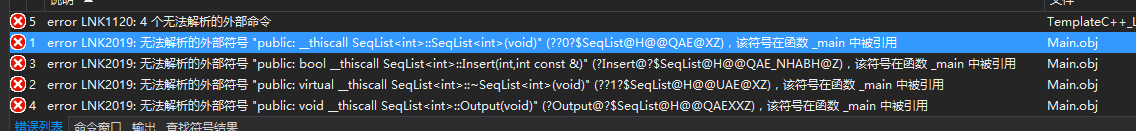
\includegraphics[width = 14cm]{MustKnowError.png}
			\caption{Error: 没包含cpp文件}
		\end{figure}
		
	\textbf{解决方法}:同时包含.cpp与.h文件,或将实现写入.h文件
		\begin{figure}[h]
			\centering
			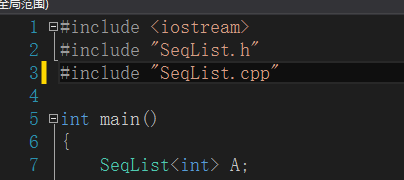
\includegraphics[scale = 0.6]{TemplateFirst.png}
			\caption{解决LNK2019 问题}
		\end{figure}	
 
 
\section{函数模版}
	\subsection{概述}
		函数模板定义了参数化的非成员函数,这使得程序员能够用不同类型的参数调用相同的函数,由编译器决定调用哪一种类型,并且从模板中生成相应的代码
		
		\subparagraph{定义}template<typename T> 返回类型\ 函数名\ (形参表) \ \{函数体\}
	
	\subsection{普通函数模版}
		针对于基本的单元类型
		
		\subparagraph{实现}:
	\begin{lstlisting}
	    #include <string> 
	    #include <iostream> 
	    using namespace std; 
	    template<typename T> void print(const T& var) 
	    {     
		    cout << var << endl; 
	    } 
	    int main() 
	    {     
		    string str("Hello World");     
		    const int num=1234; 
		    print(str); 
		    print(num); 
		    return 0; 
	    } 
	    //输出:Hello World  
	    //  1234,	如果不用泛型的话,这个得重新实现 	
	    
	    
///////////////////////////////////////////////////////////////////////
	    // 定义函数模板,找出三个值中最小的值,与数据类型无关 
	    template <class T> 
	    T min(T ii, T jj, T kk) 
	    { 
		    T temp; 
		    if((ii<jj)&&(ii<kk)){temp=ii;} 
		    else if((jj<ii)&&(jj<kk)){temp=jj;} 
		    else{    temp=kk; } 
		    return temp; 
	    } 
	    // 下面是主函数 
	    void main() 
	    { 
		    cout<<min(100,20,30)<<endl; 
		    cout<<min(10.60,10.64,53.21)<<endl; 
		    cout<<min('c','a','C')<<endl; 
		    cout<<min("anderson","Washington","Smith")<<endl; //非单元类型,会导致异常结果,
		    /*
			    a-z:97-122
			    A-Z:65-90
			    0-9:48-57
			    
			    所以最小的应该为Smith
		    */
	    }     
	\end{lstlisting}	
	
	\subsection{定制非模版函数(重载函数模版)}
		函数模板功能非常强大,但是有时候可能会陷入困境,加入待比较的函数模板没有提供正确的操作符,或者提供的操作对某些特定的类型会产生不正确的操作结果,则程序不会对此进行编译。为了避免这种错误,可以使用函数模板和同名的非模板函数重载,这就是\textbf{函数定制},以完成对特定的类型等完成特定的功能.
		
		函数模板与同名的非模板函数重载必须遵守以下规定:
		\begin{itemize}[itemindent = 1em]
			\item 寻找一个参数完全匹配的\textbf{函数},如有,则调用它
			\item 如果失败,寻找一个\textbf{函数模板},使其实例化,产生一个匹配的模板函数,若有,则调用它
			\item 如果失败,再试低一级的对函数重载的方法,例如通过类型转换可产生的参数匹配等,若找到匹配的函数,调用它
		\end{itemize}
	\begin{lstlisting}
	// 定义函数模板,找出三个值中最小的值,与数据类型无关 
	template <class T> 
	T min(T ii, T jj, T kk) 
	{ 
		T temp; 
		if((ii<jj)&&(ii<kk)){        temp=ii;    } 
		else if((jj<ii)&&(jj<kk)){        temp=jj;    } 
		else    {        temp=kk;    } 
		return temp; 
	} 
	//非模板函数重载 
	const char* min(const char* ch1, const char* ch2,const char* ch3) 
	{ 
		const char* temp; 
		int result1 = strcmp(ch1,ch2); 
		int result2 = strcmp(ch1,ch3); 
		int result3 = strcmp(ch2,ch1); 
		int result4 = strcmp(ch2,ch3); 
		if((result1<0)&&(result2<0))    {        temp = ch1;    } 
		else if((result3<0)&&(result4<0))    {        temp=ch2;    } 
		else    {        temp=ch3;    } 
		return temp; 
	} 
	void main() 
	{ 
		cout<<min(100,20,30)<<endl; 
		cout<<min(10.60,10.64,53.21)<<endl; 
		cout<<min('c','a','C')<<endl;     
		cout<<min("anderson","Washington","Smith")<<endl; //正常输出 Smith
	} 	
	\end{lstlisting}
	
	\subsection{实参的演绎-模版类型推导确定}
		
		当我们调用某些模版时,模板参数可以由我们所传递的实参来决定。如下
	\begin{lstlisting}
		template <typename T>
		inline T const& max(T const& a, T const& b);
		
		max(4,7);		//Ok: 两个实参的类型都是int
		max(4,4.2);		//ERROR: 第一个T为int,第二个T为double
	\end{lstlisting}
	
	有三种方法可以处理上面的错误:
	\begin{enumerate}[itemindent = 1em]
		\item 对实参进行强制类型转换,使他们可以相互匹配: max(static\_cast<double>(4),4.2);
		\item 显示指定T的类型:max<double>(4,4.2); 
		\item 指定两个参数可以具有不同的类型
	\end{enumerate}
\section{类模板}



\section{非类型模版参数}
	\verb|template<class T, size_t N> class Stack{};|
	\begin{lstlisting}
	template<class T, size_t N> class Stack{
		T data[N]; // Fixed capacity is N
		size_t count;
		
	public:
		void push(const T& t);
	};
	
	template<class T>
	inline void Stack<T>::push(const T& t){// Something}
	\end{lstlisting}

\section{默认模版参数}
	\verb|template<class T, size_t N = 100> class Stack{};|
	
	\begin{lstlisting}
	template<class T = int, size_t N = 100>
	class Stack{
		T data[N];
		size_t count;
	public:
		void push(const T& t);
	};
	
	Stack<> myStack; 	// Same as Stack<int, 100>
	\end{lstlisting}
	
\section{模版类型的模版参数}
	\verb|template<class T, template<class U> class Seq> class Container{};|
	
	\begin{lstlisting}
	template<class T, template<class U> class Seq>
	class Container{
		Seq<T> seq;
	public:
		void append(const T& t){seq.push_back(t);}
		// Other Stuffs
	};
	
	Container<int, vector> container;
	\end{lstlisting}
	
\section{typename}
	 必须 对 \textbf{模版中的嵌套 类型}使用 \verb|typename|进行说明,否则模版会编译不过
	\begin{lstlisting}
	template<class T, template<class U, class = allocate<U> > class Seq>
	void printSeq(const Seq<T>& seq)
	{
		for(typename Seq<T>::iterator b = seq.begin(); b != seq.end();)
		{
			cout<< *b++ <<endl;
		}
	}
	\end{lstlisting}
	
	\subsection{模板类中再有模版成员}
		\begin{lstlisting}
	template<typename T> class complex{
		template<class X> complex(const complex<X>&);
	};
	
	complex<float> z(1,2);
	complex<double> w(z);
	
	int data[5] = {1, 2, 3, 4, 5};
	vector<int> v1(data, data+5);
	vector<double> v2(v1.begin(),v1.end());
		\end{lstlisting}
		
\section{模版特化}
	\subsection{Full Specialization}
		\verb|template<>|
		\begin{lstlisting}
// 函数特化
	template<class T> const T& min(const T& a, const T& b)
	{
		return (a<b) ? a:b;
	}
	
	// An explicit sepcialization of the min template
	template<>
	const char* const& min<const char*> (const char* const& a, const char* const& b)
	{
		return (strcmp(a,b) < 0) ? a : b;
	}
	
// 类特化
	template<class T, class Allocator = allocator<T> > class vector{};
	
	template<> class vector<bool, allocator<bool> >{};	
		\end{lstlisting}
	\subsection{Partial Specialization}
		改变多模版参数的一个为固定值,或同类型的指针类型,然后特化函数

\section{模版友元}
	\begin{lstlisting}
	// Necessary forward Declarations;
	template<class T> class Frinedly;
	template<class T> void f(const Friendly<T> &);
	
	template<class T> class Friendly
	{
		T t;
	public:
		Friendly(const T& theT):t (theT){}
		// f后的<> 必不可少,要不就是普通函数而不是模版函数了
		friend void f<>(const Friendly<T>&);
		void g(){ f(*this); }
	}
	
	
	// 特化 友元
	
	template<class T> class Friendly
	{
		template<class U> friend void f<>(const Friendly<U>&);
		/*
			由于友元声明的模版参数独立于T,因此任意的T和U的组合都允许使用,形成友元关系
			
			像成员模版一样,友元模版也可以出现 在 非模版类中。
		*/
	}
	\end{lstlisting}	
\section{参考}\url{http://developer.51cto.com/art/201208/351569.htm}    

\chapter{Effective}
	\section{Effective C++}
		\subsection{C++ 基本相关性能提升}
		\paragraph{1.尽量以const,enum,inline替换\#define} 编译过程:\verb|.c|文件--预处理-->\verb|.i|文件--编译-->\verb|.o|文件--链接-->\verb|bin|文件
		
		多了类型检查,因为\verb|#define| 只是单纯的替换
		\paragraph{2.尽可能使用const} const允许你告诉编译器和其他程序员某值应保持不变,\textbf{只要“某值”确实是不该被改变的,那就该确实说出来}。
		\paragraph{3.确定对象被使用前已先被初始化}
			\subparagraph{赋值与初始化} C++规定,对象的成员变量的初始化动作发生在进入构造函数本体之前。所以应将成员变量的初始化置于构造函数的初始化列表中
			
			\begin{lstlisting}
ABEntry::ABEntry(const std::string& name, const std::string& address,
const std::list<PhoneNumber>& phones)
{ 
	theName = name;                //这些都是赋值,而非初始化
	theAddress = address;          //这些成员变量在进入函数体之前已调用默认构造函数,接着又调用赋值函数,
	thePhones = phones;            //即要经过两次的函数调用。            
	numTimesConsulted = 0;
} 
	 
ABEntry::ABEntry(const std::string& name, const std::string& address,
const std::list<PhoneNumber>& phones) 
:theName(name),                    //这些才是初始化 
 theAddress(address),                //这些成员变量只用相应的值进行拷贝构造函数,所以通常效率更高。
 thePhones(phones),
 numTimesConsulted(0){} 
			\end{lstlisting}
				
			\subparagraph{Note}  C++有着十分固定的“成员初始化次序”。\textbf{基类总是在派生类之前被初始化},而\textbf{类的成员变量总是以其说明次序被初始化}。所以:\verb|当在成员初始化列表中列各成员时,最好总是以其声明次序为次序|。
		\subsection{C++ 构造/析构/赋值性能提升}
		\paragraph{4.C++默认编写并调用哪些函数} 如果你\textbf{自己没声明},\textbf{编译器就会}为类声明(编译器版本的)一个\textbf{拷贝构造}函数,一个\textbf{拷贝赋值操作符}和一个\textbf{析构}函数。此外\textbf{如果你没有声明任何构造函数},\textbf{编译器也会}成为你声明一个默认构造函数。所有这些函数都是\verb|public|且\verb|inline|,编译器产生规则如下:

			\begin{itemize}
				\item \verb|调用准则|:\textbf{惟有}当这些函数\textbf{被需要}(被调用),它们才会被编译器创建出来。即有需求,编译器才会创建它们。
				\item \verb|析构函数|:\textbf{编译器产生的析构函数}是个\verb|non-virtual|,\textbf{除非}这个类的\textbf{基类自身声明有}\verb|virtual|析构函数
				\item \verb|拷贝构造|:至于\textbf{拷贝构造函数和拷贝赋值操作符},编译器创建的版本\textbf{只是单纯地}\textit{将}来源对象的\textbf{每一个非静态成员变量}\textit{拷贝到}目标对象 (\verb|浅拷贝|)
				\item \verb|构造函数|:如一个类\textbf{声明了一个构造函数}(无论有没参数),编译器\textbf{就不再为}它创建默认构造函数
			\end{itemize}
				
		\paragraph{5.若不想使用编译器自动生成的函数,就该明确拒绝} 为驳回编译器自动(暗自)提供的机能,可将相应的成员函数声明为\verb|private|并且不予实现。使用像\verb|noncopyable|这样的基类也是一种做法, 除此C++11 提供\verb|=delete| 关键字可以完成该操作。
			
		\paragraph{6.为多态基类声明virtual析构函数} 当基类的指针指向派生类的对象的时候,当我们使用完,对其调用\verb|delete|的时候,其结果将是未有定义——基类成分通常会被销毁,而派生类的充分可能还留在堆里。这可是形成资源泄漏、败坏之数据结构、在调试器上消费许多时间
			
			消除以上问题的做法很简单:给基类一个\verb|virtual|析构函数。此后删除派生类对象就会如你想要的那般。
			
			 \verb|STL容器|都不带\verb|virtual|析构函数,所以最好别派生它们
			 
		\begin{lstlisting}[frame = lbrT,xleftmargin=.02\textwidth]
// Note:
1、带有多态性质的基类应该声明一个virtual析构函数。如果一个类带有任何virtual函数,它就应该拥有一个virtual析构函数

2、一个类的设计目的不是作为基类使用,或不是为了具备多态性,就不该声明virtual析构函数
		\end{lstlisting}
				 
		\paragraph{7.别让异常逃离析构函数} 析构函数绝对不要吐出异常。如果一个被析构函数调用的函数可能抛出异常,析构函数应该捕捉任何异常,然后吞下它们(不传播)或结束程序
		
		\paragraph{8.决不让构造和析构过程中调用virtual函数} 基类的构造函数的执行要早于派生类的构造函数,当基类的构造函数执行时,派生类的成员变量尚未初始化。派生类的成员变量没初始化,即为指向虚函数表的指针\verb|vptr|没被初始化又怎么去调用派生类的\verb|virtual|函数呢?析构函数也相同,派生类先于基类被析构,又如何去找派生类相应的虚函数?
		
		\paragraph{9.令operator= 返回一个reference to *this}
			对于赋值操作符,我们常常\textbf{要达到}这种类似效果,即\textbf{连续赋值}
			\begin{lstlisting}[xleftmargin=.04\textwidth]
 int x, y, z;
 x = y = z = 15;
 
 赋值采用右结合律,所以上述连锁赋值被解析为
 x = (y = (z = 15));
 这里15先被赋值给z,然后其结果(更新后的z) 再赋值给y,然后其结果(更新后的y)再赋值给x.
			\end{lstlisting}
			
			为了实现“连锁赋值”,赋值操作符必须\textbf{返回一个“引用”}指向操作符的左侧实参,这个协议适合所有的赋值运算。
			\begin{lstlisting}[xleftmargin=.04\textwidth]
Widget&  operator = (const Widget &rhs)
{
	...
	return *this;
}

class Widget{
public:
	Widget& operator+=(const Widget& rhs)   //这个协议使用于所有赋值相关运算 (+=, -=, *=等)
	{
		...
		return *this;
	}
	
	Widget& operator= (int rhs)
	{
		...
		return *this;
	}
};
			\end{lstlisting}
		\paragraph{10.在operator =中处理“自我赋值”}
			自我赋值如下所示:
		\begin{lstlisting}
Widget w;
w = w;
a[i] = a[j]; //i == j or i != j
*px = *py;	 // px,py指向同个地址;
		\end{lstlisting}
		
		\begin{lstlisting}
// 该怎么做
Widget& Widget::operator=(const Widget& rhs)
{ 
	Widget temp(rhs);
	swap(temp);
	return *this;
} 
		\end{lstlisting}
		
		“许多时候一群精心安排的语句就可以导出异常安全(\verb|new| 新对象时出错,那么原来的东西亦将不复存在)(自我赋值)的代码。”以下note给出正确做此事的规矩.
		\begin{lstlisting}[frame = lbrT]
1、确保当对象自我赋值时operator =有良好行为。其中技术包括比较“来源对象”和“目标对象”的地址、精心周到的语句顺序、以及copy-and-swap
2、确定任何函数如果操作一个以上的对象,而其中多个对象是同一个对象时,其行为仍然正确
		\end{lstlisting}	
				
		\paragraph{11.复制对象时勿忘其每一个成员} 如果你为class \textbf{添加一个成员变量},你必须同时修改 复制构造函数 和 赋值操作符函数,当\textbf{使用继承时},子类需重写 拷贝构造,且\textbf{不要忘了基类的成分}
		
			\begin{lstlisting}
PriorityCustomer::PriorityCustomer(const PriorityCustomer& rhs)
: 	Customer(rhs), 			// 调用 Base类的拷贝构造函数
	priority(rhs.priority)
{
	logCall("PriorityCustomer Copy constructor");
}

PriorityCustomer& operator=(const PriorityCustomer& rhs)
{
	Customer::operator=(rhs);  	// 对Base  类成分进行赋值动作
	priority = rhs.priority;
	return (*this);
}
			\end{lstlisting}
		

	\subsection{资源管理}
		\paragraph{12.以对象管理资源} 使用\verb|shared_ptr| 等代理对象管理指针
		\paragraph{13.在资源管理类中小心拷贝行为}
		\paragraph{14.在资源管理类中提供对原始资源的访问}
		\paragraph{15.成对使用new和delete时要采取相同形式}
		\paragraph{16.以独立语句将newed对象置入智能指针}
	\subsection{设计与声明}
		\paragraph{17.让接口容易被正确使用,不易被误用}
		\paragraph{18.设计class犹如设计type}
		\paragraph{19.宁以pass-by-reference-to-const替代psss-by-value} 这种传递方式效率高得多:没有任何构造函数或析构函数被调用,因为没有任何新对象被创建。
		
		\paragraph{20.必须返回对象时,别妄想返回其reference}
			函数创建新对象的途径有二:在栈空间和堆空间
			
			\begin{itemize}
				\item \textbf{栈上}:即在函数内的局部变量。局部变量在函数返回后就没有存在的意义,若还对它“念念不忘”,将带来灾难性后果。所以传引用在栈上不可行
				\item \textbf{堆上}:在堆上构造一个对象,并返回。看似可行,也埋下了资源泄漏的危险。谁该对这对象实施delete呢?别把这种对资源的管理寄托完全寄托于用户。所以传引用在堆上不可行
				\item \textbf{静态对象}:出于我们对多线程安全性的疑虑,以及当线程中两个函数对单份对象的处理也可能带来不可测行为。所以静态对象也是不可行的
			\end{itemize}
			
			一个“必须返回新对象”的函数的正确写法是:就让那个函数返回一个新对象
		\paragraph{21.将成员变量声明为private}
		\paragraph{22.宁以non-member、non-friend替换member函数} 这样做可以增加封装性、包裹弹性和\textbf{机能扩充性}
		\paragraph{23.若所有参数皆需类型转换,请为此采用non-member函数}
		\paragraph{24.考虑写出一个不抛异常的swap函数}
	\subsection{实现}
		\paragraph{25.尽可能延后变量定义式的出现时间}
		\paragraph{26.尽量少做转型动作}
		\paragraph{27.避免返回handls指向对象内部成分}
		\paragraph{28.为“异常安全”而努力是值得的}
		\paragraph{29.透彻了解inlining的里里外外}
		\paragraph{30.将文件间的编译依存关系降至最低}
	\subsection{继承与面向对象设计}
		\paragraph{31.确定你的public继承塑模出is-a关系}
		\paragraph{32.避免遮掩继承而来的名称}
		\paragraph{33.区分接口继承和实现继承}
			\verb|public|继承分为:1、\verb|接口继承|2、\verb|实现继承|
			\begin{itemize}
				\item 成员函数的接口总是会被继承
				\item 声明一个\textbf{纯虚函数}的目的是为了\textbf{让派生类继承函数接口}-\verb|"变化性"|
				\item 声明一个\textbf{虚函数}的目的是\textbf{让派生类继承该函数的接口和缺省实现}-\verb|"不变性,与变化性"|
				\item 声明一个\textbf{非虚函数}的目的是\textbf{为了令派生类继承函数的接口及一份强制性实现}-\verb|"不变性,凌驾特异性"|
			\end{itemize}
		\paragraph{34.考虑virtual函数以外的其它选择}
		\paragraph{35.绝不重新定义继承而来的non-virtual函数}
		\paragraph{36.绝不重新定义继承而来的缺省参数值}
		\paragraph{37.通过符合塑模出has-a或“根据某物实现出”}
	\section{More Effective C++}
		\subsection{基础议题(Basics)}
			\paragraph{1.仔细区别 pointers 和 references}
				在任何情况下都\textbf{不能使用}\textit{指向空值}的\textbf{引用}。一个引用必须总是指向某些对象。在C++里,引用应被初始化,不存在指向空值的引用这个事实意味着使用引用的代码效率比使用指针的要高。因为在使用引用之前不需要测试它的合法性。
				
				指针与引用的另一个重要的不同是指针可以被重新赋值以指向另一个不同的对象。但是引用则总是指向在初始化时被指定的对象,以后不能改变
				
				总的来说,在以下情况下你应该\textbf{使用指针},\textit{一是}你考虑到存在不指向任何对象的可能(在这种情况下,你能够设置指针为空),\textit{二是}你需要能够在不同的时刻指向不同的对象(在这种情况下,你能改变指针的指向)。如果总是指向一个对象并且一旦指向一个对象后就\textit{不会改变指向},那么你应该\textbf{使用引用}。
				还有一种情况,就是当你\textbf{重载某个操作符}时,你应该使用引用
			\paragraph{2.最好使用 C++ 转型操作符}
				\verb|static_cast<double>(value)|
				
			\paragraph{3.绝对不要以多态方式处理数组} 继承 后仍然使用 基类数组,导致数组的下标运算出现问题,因为数组是根据元素的sizeof 进行计算下一个元素出现的位置,如果派生类的 sizeof 值不同,将会出现内存错误。
				\begin{lstlisting}
	#include <iostream>
	using namespace std;
	
	struct B
	{
		virtual void print() const{cout<<"base print()"<<endl;}
	};
	struct D : B
	{
		void print() const{cout<<"derived print()"<<endl;}
		int id;  //如果没有此句,执行将正确,因为基类对象和子类对象长度相同  
	};
	
	int fun(const B array[],int size)
	{
		for(int i = 0;i<size;++i)
		{
			array[i].print();
		}
	}
	
	int main()
	{
		B barray[5];
		fun(barray,5);
		D darray[5];
		fun(darray,5);
	}
				\end{lstlisting}
			\paragraph{4.避免无用的 default constructors}
			
		\subsection{操作符(Operators)}
			\paragraph{5.对定制的“类型转换函数”保持警觉}
				\textbf{定义类似功能的函数},而抛弃隐式类型转换,\textbf{使得类型转换必须显示调用}。例如 \verb|String|类没有定义对\verb|Char*|的隐式转换,而是用\verb|c_str|函数来实施这个转换。拥有单个参数(或除第一个参数外都有默认值的多参数)构造函数的类,很容易被隐式类型转换,最好加上 \verb|explicit| 防止\textbf{隐式类型转换}
				
				\subparagraph{隐身类 类型抓换}
					\begin{itemize}
						\item  可以用 \textbf{单个形参来调用} 的构造函数定义了\textit{从} \textbf{形参类型 到 该类类型} 的一个隐式转换,这里应该注意的是, “可以用单个形参进行调用” 并不是指构造函数只能有一个形参,而是它可以有多个形参,但那些形参都是有默认实参的。
						\begin{lstlisting}
	#include <string>
	#include <iostream>
	using namespace std ;
	class BOOK  //定义了一个书类
	{
	private:
		string _bookISBN ;  //书的ISBN号
		float _price ;    //书的价格
	
	public:
		//定义了一个成员函数,这个函数即是那个“期待一个实参为类类型的函数”
		//这个函数用于比较两本书的ISBN号是否相同
		bool isSameISBN(const BOOK & other ){
			return other._bookISBN==_bookISBN;
		}
	
		//类的构造函数,即那个“能够用一个参数进行调用的构造函数”(虽然它有两个形参,但其中一个有默认实参,只用一个参数也能进行调用)
		BOOK(string ISBN,float price=0.0f):_bookISBN(ISBN),_price(price){}
	};
	
	int main()
	{
		BOOK A("A-A-A");
		BOOK B("B-B-B");
		
		cout<<A.isSameISBN(B)<<endl;   //正经地进行比较,无需发生转换
		
		cout<<A.isSameISBN(string("A-A-A"))<<endl; //此处即发生一个隐式转换:string类型-->BOOK类型,借助BOOK的构造函数进行转换,以满足isSameISBN函数的参数期待。
		cout<<A.isSameISBN(BOOK("A-A-A"))<<endl;    //显式创建临时对象,也即是编译器干的事情。
		
		system("pause");
	}
						\end{lstlisting}
						
							代码中可以看到,\verb|isSameISBN|函数是期待一个\verb|BOOK|类类型形参的,但我们却传递了一个\verb|string|类型的给它,这不是它想要的啊!还好,\verb|BOOK|类中有个构造函数,它使用一个\verb|string|类型实参进行调用,编译器调用了这个构造函数,隐式地将\verb|stirng|类型转换为\verb|BOOK|类型(构造了一个BOOK\textbf{临时对象}),再传递给\verb|isSameISBN|函数。
							
							隐式类类型转换还是会带来风险的,正如上面标记,\textbf{隐式转换得到类的临时变量,完成操作后就消失了},我们构造了一个完成测试后被丢弃的对象。
						\item 隐式类型转换运算符只是一个样子奇怪的成员函数:\verb|operator| \textbf{关键字},其后跟一个类型符号。你不用定义函数的返回类型,因为返回类型就是这个函数的名字。例如\textbf{为了允许}\verb|Rational|(有理数)类\textbf{隐式地转换为}\verb|double|类型(在用有理数进行混合类型运算时,可能有用),你\textbf{可以如此声明}\verb|Rational|类
						
						\begin{lstlisting}
	class Rational {
	public:
		...
		operator double() const; // 转换Rational类成 double类型
	}; 
	
	Rational r(1, 2); // r 的值是1/2
	double d = 0.5 * r; // 隐式转换 r 到double,
						\end{lstlisting}
					\end{itemize}
				
				\subparagraph{避免 隐身转换}	一般来说,越有经验的C++程序员就越喜欢避开类型转换运算符。例如在\verb|C++|标准库委员会工作的人员是在此领域最有经验的,他们加在库函数中的\verb|string|类型没有包括隐式地从\verb|string|转换成C风格的\verb|char*|的功能,而是定义了一个成员函数\verb|c_str|用来完成这个转换,这是巧合么?我看不是。
					\begin{itemize}
						\item 声明装换功能的函数,如\verb|string| 的\verb|c_str()|函数
						\item \verb|explicit operator Type() const;|
						\item \verb|explicit BOOK(string ISBN,float price=0.0f);|
					\end{itemize}
					
			\paragraph{6.区别 increment/decrement 操作符的前置和后置形式}
			\paragraph{7.千万不要重载 \&\&, || 和 , 操作符}
			\paragraph{8.了解各种不同意义的 new 和 delete}
				\subparagraph{new操作符(new operator)和new操作(operator new)的区别}
					当你写这样的代码:
					\verb|string *ps = new string("Memory Management");|
					你使用的\verb|new是new操作符|。这个操作符就象\verb|sizeof|一样是语言内置的,你不能改变它的含义,它的功能总是一样的。它要完成的功能分成两部分。\textbf{第一部分}是分配足够的内存以便容纳所需类型的对象。\textbf{第二部分}是它调用构造函数初始化内存中的对象。new操作符总是做这两件事情,你不能以任何方式改变它的行为。
					
					你所能改变的是如何为对象分配内存。\verb|new|操作符调用一个函数来完成必需的内存分配,你能够重写或重载这个函数来改变它的行为。\verb|new|操作符为分配内存所调用函数的名字是\verb|operator new|。
					函数\verb|operator new| 通常这样声明:
					\verb|void * operator new(size_t size);|
					
					就象\verb|malloc|一样,\verb|operator new|的职责\textbf{只是分配内存}。它对构造函数一无所知。
			
				\subparagraph{placement new}
		\subsection{异常(Exceptions)}
			\paragraph{--堆栈辗转开解stack-unwinding}如果一个函数中出现异常,在函数内即通过 \verb|try..catch| 捕捉的话,可以继续往下执行;如果不捕捉就会抛出(或通过 \verb|throw |显式抛出)到外层函数,则当前函数会终止运行,释放当前函数内的局部对象(局部对象的析构函数就自然被调用了),外层函数如果也没有捕捉到的话,会再次抛出到更外层的函数,该外层函数也会退出,释放其局部对象……如此一直循环下去,直到找到匹配的 catch 子句,如果找到 main 函数中仍找不到,则退出程序。
			
			\paragraph{9.利用 destructors 避免泄漏资源}
			\paragraph{10.在 constructors 内阻止资源泄漏} 使用智能指针 在初始化列表中进行初始化 堆上资源可以防止 异常情况下的资源泄漏,\textbf{其实,防止内存泄漏就用 智能指针的手段就可以了}
			
			\paragraph{11.禁止异常流出 destructors 之外}
				这一条讲得其实是捕获析构函数里的异常的重要性。第一是防止程序调用 \verb|terminate| 终止(这里有个名词叫:堆栈辗转开解 \verb|stack-unwinding|);第二是析构函数内如果发生异常,则异常后面的代码将不执行,无法确保我们完成我们想做的清理工作。
				
				之前我们知道,析构函数被调用,会发生在对象被删除时,如栈对象超出作用域或堆对象被显式 \verb|delete| (还有继承体系中,virtual 基类析构函数会在子类对象析构时调用)。除此之外,在异常传递的堆栈辗转开解(\verb|stack-unwinding|)过程中,异常处理系统也会删除局部对象,从而调用局部对象的析构函数,而此时如果该析构函数也抛出异常,C++程序是无法同时处理两个异常的,就会调用 \verb|terminate()|终止程序(会立即终止,连局部对象也不释放)。另外,如果异常被抛出,析构函数可能未执行完毕,导致一些清理工作不能完成。
				
				所以不建议在析构函数中抛出异常,如果异常不可避免,则应在析构函数内捕获,而不应当抛出
				
			\paragraph{12.了解 "抛出一个 exception ”  与 “传递一个参数” 或 “调用一个虚函数”之间的差异}
			\paragraph{13.以 by reference 方式捕捉 exceptions} 提高效率
			
			\paragraph{14.明智运用 exception specifications} 毫无疑问,异常规格是一个引人注目的特性。它使得代码更容易理解,因为它明确地描述了一个函数可以抛出什么样的异常
			\paragraph{15.了解异常处理的成本}
			
		\subsection{效率(Efficiency)}
			\paragraph{16.谨记 80-20 法则}
			\paragraph{17.考虑使用 lazy evaluation(缓式评估)}
			\paragraph{18.分期摊还预期的计算成本}
			\paragraph{19.了解临时对象的来源}
			\paragraph{20.协助完成“返回值优化(RVO)}
			\paragraph{21.利用重载技术避免隐式类型转换}
			\paragraph{22.考虑以操作符复合形式(op=)取代其独身形式(op)}
			\paragraph{23.考虑使用其它程序库}
			\paragraph{24.了解 virtual functions、multiple inheritance、virtual base classes、runtime type identification 的成本 }
			
		\subsection{技术(Techniques,Idioms,Patterns)}
			\paragraph{25.将 constructor 和 non-member functions 虚化}
			\paragraph{26.限制某个 class 所能产生的对象数量}
			\paragraph{27.要求(或禁止)对象产生于 heap 中}
			\paragraph{28.Smart Pointer(智能指针)}
			\paragraph{29.Reference counting(引用计数)}
			\paragraph{30.Proxy classes(替身类、代理类)}
			
		\subsection{杂项讨论(Miscellany)}
			\paragraph{31.在未来时态下发展程序}
			\paragraph{32.将非尾端类设计为抽象类}	
				
	\section{Effective Modern C++}
		\subsection{Deducing Types}
		\subsection{auto}
		\subsection{Moving to Modern C++}
		\subsection{Smart Pointers}
		\subsection{Rvalue References, Move Semantics, and Perfect Forwarding}
		\subsection{Lambda Expressions}
		\subsection{The Concurrency API}
		\subsection{Tweaks}
	\section{Effective STL}
		\subsection{容器}
			\paragraph{1.慎重选择容器类型,根据需要选择高效的容器类型}
			\paragraph{2.不要试图编写独立于容器类型的代码}
			\paragraph{3.确定容器中的对象拷贝正确而高效。也就是防止在存在继承关系时发生剥离}
			\paragraph{4.调用empty而不是检查size()是否为0来判断容器是否为空} 原因是调用\verb|empty|比检查size()更加高效
			\paragraph{5.尽量使用区间成员,而不是多次使用与之对应的单元素成员函数,原因是这样更加高效} 如尽量使用\verb|vector|的\verb|assign|或\verb|insert|成员函数,而不是一直使用\verb|push_back|
			\paragraph{6.小心C++编译器最烦人的分析机制}
			\paragraph{7.如果在容器中包含了能过new操作创建的指针,切记在容器对象析构前将指针delete掉} 使用智能指针如\verb|shared_ptr|(C++11)是个比较好的选择
			\paragraph{\sout{8.切勿创建包含auto\_ptr的容器对象}} \verb|auto_ptr|不是采用引用计数实现的,放进容器中就等着出问题吧,特别是当对容器使用\verb|sort|这类会对元素进行赋值的算法之后
			
			\paragraph{9.慎重选择删除元素的方法} 这一点很重要,因为在删除一个元素之后会导致一些迭代器、指针及引用失效。所以如果手写循环删除元素一定要小心。最好的方法是\verb|vector、string、deque|采用\verb|erase-remove|这样的习惯写法,方便又安全,\verb|list|应当使用成员函数\verb|remove|,\textbf{关联容器}使用成员函数\verb|erase|。
				
			要小心的一点是算法\verb|remove|并不是真正的删除容器中的元素,因为它没有这个能力,它只能将无用的元素移去末尾。之后你必须用成员函数\verb|erase|删除无用区间
			\paragraph{10.了解分配器allocator的约定和限制}
			\paragraph{11.理解自定义分配器合理用法}
			\paragraph{12.切勿对STL容器的线程安全性有不切实际的依赖} 请手工保证线程安全,不要依赖\verb|STL|
		\subsection{vector And string}
			\paragraph{13.尽量用vector和string代替动态分配的数组}
			\paragraph{14.使用reserve来避免不必要的内存重新分配} 成员函数\verb|reserve|可以为容器预留一块内存,当容器大小(size)增大时,\textbf{不用重新分配内在,可以提高效率}。需要缩减分配的内存时可以使用后面提到的\verb|swap技术|,或者使用成员函数\verb|.shrink_to_fit|
			
			\paragraph{15.注意string实现的多样性}
			\paragraph{16.了解如何把vector和string数据传给旧的C API} \verb|vector|请使用 \verb|&vector[0]|,当然先要确定容器不为空。\verb|string|使用\verb|c_str()|方法
			
			\paragraph{17.使用“swap 技巧”除去多余的容量} 与临时变量交换,然后利用 临时变量的 RAII 机制,保证了在任何情况下,使用对象时先构造对象,最后析构对象。从而在析构该临时对象时 将空间释放掉
			
			\paragraph{18.避免使用vector<bool>} 因为它不是容器,它是用位来存储\verb|bool|值的,所以它也没有迭代器,不能对其使用标准算法。最好使用\verb|deque <bool> 或bitset|代替之
			
		\subsection{关联容器}
			\paragraph{19.理解相等equality 和等价equivalence 的区别} 在实际中相等的概念是基于 \verb|operator==| 的。\verb|find|对“相同”的定义是相等,是以 \verb|operator==|为基础的; \verb|set::instert|对“相同”的定义是等价,是以\verb|operator< |为基础的
			
			\paragraph{20.为包含指针的关联容器指定比较类型}	默认情况的比较类型是 \verb|less<T>|,所以\textbf{只会比较指针的值},\textit{而不是}\textbf{指针指向的值},所以需要手工指定比较类型,以比较指针指向的值。
			
			\paragraph{21.总是让比较函数在等值情况下返回false} 特别是在关联容器基于比较函数判断等价的情况下。否则会导致相同的值按照定义是不等价的
			\paragraph{22.切勿直接修改set 或 multiset中的键} 会破坏该数据结构。而\verb|map|中的键被\verb|const|修饰,不能更改
			\paragraph{23.考虑用排序的vector 替代 关联容器}
			\paragraph{24.当效率至关重要时,请在map::operator[]与map::insert之间做出谨慎选择} 选择的标准是:当向\verb|map|中添加元素时,要优先选择\verb|insert|; 当更新已经在\verb|map|中的元素的值时,要优先选择\verb|operator[]|
			\paragraph{25.熟悉散列容器} \verb|unordered_map、unordered_multimap、unordered_set、unordered_multiset|
		\subsection{迭代器}
			\paragraph{26.尽量使用iterator,而不是const\_iterator、reverse\_iterator及const\_reverse\_iterator} 使用\verb|iterator|会减少很多麻烦,所以使用STL时尽量使用\verb|iterator|
			
			\paragraph{27.使用distance和advance将容器的const\_iterator转换成iterator} 首先明确的是不能使用\verb|const_cast|进行转换,因为这两个根本就是两个完全不相关的类,比\verb|string和complex<double>|之间的关系还远。可以使用下面的技术转换,\verb|i是iterator|类型,\verb|ci是const_iterator|类型:
			
				\begin{lstlisting}
typedef IntDeque::const_iterator ConstIter;
advance(i, distance<ConstIter>(i, ci));   // <ConstIter> 不能少,否则编译通不过
				\end{lstlisting}
			\paragraph{28.正确理解由reverse\_iterator的base()成员函数所产生的iterator的用法} 向右有一个位置的偏移,保证了对于插入操作而言,\verb|ri和ri.base()|是等价的
			
			对于删除而言则不是等价的,要先\verb|++ri|,如\verb|v.erase((++ri).base())|;	
			\paragraph{29.对非格式化的逐个字符的输入考虑使用 istreambuf\_iterator} 比\verb|istream_iterator|效率更高而且更方便(不用清\verb|iOS::skipws|标志)。相对的还有\verb|ostreambuf_iterator|
		\subsection{算法}
			\paragraph{30.确保目标区间足够大}:
			
			\verb|transform(values.begin(), values.end(), results.end(), transmogrify); |
			
			可以更改为
			
			\verb|transform(values.begin(), values.end(), back_inserter(results), transmogrify);|
			
			应该使用插入迭代器。插入迭代器有 \verb|inserter|、\verb|back_inserter|、\verb|front_inserter|、\verb|ostream_iterator|
			\paragraph{31.了解各种与排序有关的选择}
				\subparagraph{非稳定排序}都要求随机访问迭代器 \verb|RandomAccessIterator| 
					\begin{itemize}[itemindent = 1em]
						\item \verb|sort|:基于快排的排序
						\item \verb|partial_sort|:部分排序,指定排序区间
						\item \verb|nth_element|:将排序后位于前n个位置的元素放在前n个位置,但不对它们进行排序。
					\end{itemize}
				\subparagraph{稳定排序}
				
					\begin{itemize}[itemindent = 1em]
						\item \verb|stable_sort|:稳定排序,排序后等价元素的相对位置不会变
						\item \verb|list::sort|
					\end{itemize}
				\subparagraph{分割序列的算法}
					只需要双向迭代器
					\begin{itemize}[itemindent = 1em]
						\item \verb|partition|
						\item \verb|stable_partition|:不改变相同元素顺序
					\end{itemize}
			\paragraph{32.如果确实需要删除元素,则需要在remove这一类算法之后调用成员函数erase}
				算法\verb|remove|\textbf{不能真正删除元素},因为它没有这个能力,\textbf{必须调用}类似\verb|erase|这样的成员函数才行,\verb|list|的成员\verb|remove|\textbf{可以真正删除元素}。类似\verb|remove|这样的算法有\verb|remove_if、unique|
				
			\paragraph{33.对包含指针的容器使用remove这一类算法时要特别小心} 因为被“删除“的值可能也不存在于序列最后面,而是被覆盖了。与\verb|remove|算法的实现有关
			
			\paragraph{\sout{34.了解哪些算法要求使用排序区间作为参数}}
			\paragraph{\sout{35.通过mismatch或lexicographical\_compare实现简单忽略大小写的字符串比较}}
			
			\paragraph{36.理解copy\_if算法的正确实现}
			\paragraph{37. 使用accumulate或者for\_each进行区间统计}
		\subsection{函数子、函数子类、函数及其他}
			\paragraph{38.遵循按值传递的原则来设计函数子类} 在STL中,函数对象往往会按值传递和返回,所以在设计函数对象时要保证经过了值传递之后还能正常工作
			
			\paragraph{39.确保判别式predicate是纯函数pure function} "\verb|纯函数|"是指返回值仅仅依赖于其参数的函数
			\paragraph{40.若一个类是函数子,则就使它可配接adaptable}
			\paragraph{41.理解ptr\_fun、mem\_fun、mem\_fun\_ref的来由}
			\paragraph{42.确保 less<T>与operator< 具有相同的语义}
		\subsection{在程序中使用STL}
			\paragraph{43.算法调用优先于手写的循环}
			\paragraph{44.容器的成员函数优于同名的算法} 因为成员函数更高效,成员函数可以根据特定的容器及实现作出优化
			\paragraph{45.正确区分 count、find、binary\_search、lower\_bound、upper\_bound 和 equal\_range} 根据需要选择最高效的算法
				
				\begin{figure}[h]
					\centering
					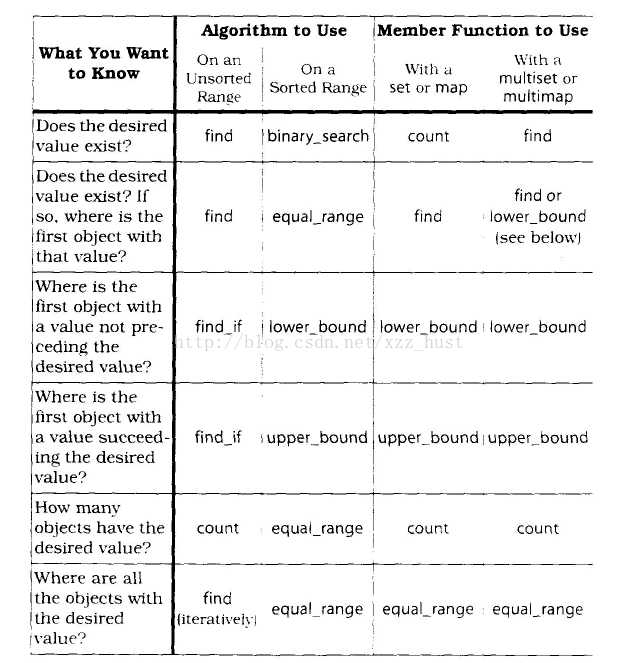
\includegraphics[scale = 0.7]{STL-Effective.png}
				\end{figure}
			\paragraph{46.考虑使用函数对象而不是函数作为STL算法参数} 一个事实是STL的sort比C语言标准中的qsort更快。原因就是sort使用函数对象,而qsort使用函数指针作为参数。\textbf{如果一个函数对象的}\verb|operator()|\textbf{已经被声明为内联的},那么其在函数体内也是内联的,但对于函数指针就不一样了,通过函数指针传递的函数不大可能会被优化成内联的,即使该函数被声明为内联的。
			
			\paragraph{47.避免产生“直写型(write-only)”代码} "直写型"代码复杂而难以理解,不便于维护。”直写型“代码就是那种一句话完成n多功能的代码,晦涩难懂。最好将”直写型“代码分解为易读的代码
			
			\paragraph{48.总是包含(\#include)正确的头文件}
			\paragraph{49.学会分析与STL相关的编译器诊断信息}

	\section{提升C++编程性能的技术}
		\subsection{跟踪范例}
			\subparagraph{关注点} 本章引入的实际问题为:定义一个简单的Trace类,将当前函数名输出到日志文件中。Trace对象会带来一定的开销,因此\textit{在默认情况}下\textbf{不会开启Trace功能}。
			
			问题是:\verb|怎么设计Trace类,使得在不开启Trace功能时引入的开销最小|
			
			\subparagraph{解决方案} 
				\begin{enumerate}
					\item \textbf{宏}:用\textbf{宏}来\verb|开关Trace功能|很简单,在不开启时开销完全没有
					\begin{lstlisting}
#ifdef TRACE
Trace trace("aaa");
#endif
					\end{lstlisting}
						
					\item \textbf{静态状态变量}:使用状态变量的话有一定的运行时开销,但能保证灵活性,是一种比较合理的选择
					\begin{lstlisting}
class Trace {
public:
	...
	static bool isTraceEnabled;
	void Debug() {
		if (isTraceEnabled) {
			...
		}
	}
}
					\end{lstlisting}
				\end{enumerate}
				
			\subparagraph{涉及技术- 延迟创建} 原本的\verb|Trace|类中内置\verb|string|成员,这样在不开启\verb|Trace|时也要承担构造和析构的开销。可以将其改为\verb|string*|,并在真正需要开启时再创建该成员。
			
			如果\verb|Trace|的开启时间远小于总时间,则此方法很有效,否则当动态创建的开销大于固定的1次构造和析构的开销时,原方法更好一些
			
		\subsection{虚函数}
		\subsection{临时对象}
			\subparagraph{关注点} 如何避免产生不必要的临时对象
			
			\subparagraph{类型不匹配} 在\textbf{不同类型间}的\textbf{赋值}容易无意中导致临时对象的创建。可以通过在单参数构造函数前加\verb|explicit|来避免这种隐式的转换产生
			
			\subparagraph{避免重复创建相同的临时对象} 临时对象有一个就够了..相同的对象的反复创建无形的增加了 工作量
				\begin{lstlisting}
Complex a;
for (int i = 0; i < 10; ++i) {
	a += 1.0;
}

其中每次循环都会创建一个值为1.0的Complex对象。可以在循环外创建一个值为1.0的Complex对象,来减少这种开销:
Complex one(1.0);
for (int i = 0; i < 10; ++i) {
	a += one;
}
				\end{lstlisting}
		\subsection{内存池}
			\subsubsection{单线程内存池}
				\subparagraph{关注点} 默认的通用内存管理器的性能在特定场景下会造成一定的性能瓶颈。本章讨论的是在单线程环境下,每次分配固定大小和不固定大小的内存时,实现比通用\verb|new/delete|性能更好的内存池管理器
				
				\subparagraph{Rational 专用内存池} 每次分配\verb|Rational|大小的内存块,用一个空闲链表维护已分配的空闲内存,在释放时重新将此内存块放回到链表中
				
				\begin{lstlisting}
class Rational {
	...
	static list<char *> freeList;
	void *operator new(size_t size) {
		if (freeList.empty()) {
			return new char[sizeof(Rational)];
		} else {
			void *buf = freeList.back();
			freeList.pop_back();
			return buf;
		}
	}
	void operator delete(void *ptr, size_t size) {
		freeList.push_back(ptr);
	}
};
				\end{lstlisting}
				
				\textbf{此版本的内存池}从不收缩,如果需要释放内存,则需要新增一个接口。
				
				\textbf{此版本的内存池}与通用内存管理器相比,收益在于:
					\begin{itemize}[itemindent = 1em]
						\item 每次分配的大小为固定值,不用在空闲列表中进行大量的查找(直接返回末端指针)。
						\item 不用处理并发情况,没有临界区						
					\end{itemize}
				
				\subparagraph{固定大小内存池实现} 不只针对Rational,而是扩展为支持任意固定大小的类:
					\begin{lstlisting}
template <typename T>
class FixedSizeMemoryPool {
public:
	FixedSizeMemoryPool(): size_(sizeof(T))
	{}
	~FixedSizeMemoryPool() {
		for(char *&p: freeList_) {
			delete[] p;
		}
	}
	void *Alloc() {
		if (freeList_.empty()) {
			return new char[size_];
		} else {
			void *buf = freeList_.back();
			freeList_.pop_back();
			return buf;
		}
	}
	void Free(void *buf) {
		freeList_.push_back(buf);
	}
private:
	list<char *> freeList_;
	const size_t size_;
};

// Rational则需要改为:
class Rational {
public:
	void *operator new(size_t size) {
		return pool.Alloc();
	}
	void operator delete(void *ptr, size_t size) {
		pool.Free(ptr);
	}
private:
	static FixedSizeMemoryPool<Rational> pool;
};
					\end{lstlisting}
				\subparagraph{不定大小内存池} 不定大小的内存池的管理方法与上面的版本不同,因为没有办法直接从链表中返回一个内存块(大小不同)。这里我们在需要时分配一个大的固定大小的内存块,每次分配单个对象的内存时就从这个内存块上分配,空间不够时就分配大的内存块。
				
				随着通用性的增加,性能也在逐渐下降。因此,在非常需要性能时,牺牲一些灵活性通用性也许会有很好的效果。
			\subsubsection{多线程内存池} 在Alloc和Free时加锁,其它保持不变

		\subsection{引用计数}
			\subparagraph{关注点} \verb|C++|使用了引用计数\textbf{来解决垃圾回收问题},基本思想是\textbf{把对象清除的责任}\textit{从}客户端代码\textbf{转移给}对象本身。
			
			引用计数可以\textbf{减少内存使用}、\textbf{避免内存泄漏},但在执行速度方面却可能会有坏处,尤其是在多线程环境中
			
			\subparagraph{引用计数的实现}方案1:
			\begin{lstlisting}
class RefCountBase {
public:
	Attach() {
		++refCount_;
	}
	Detach() {
		if (--refCount_ == 0) {
			delete this;
		}
	}
protected:
	RefCountBase(): refCount_(0) {}
	RefCountBase(const RefCountBase &rc): refCount_(0) {}
	RefCountBase &operator=(const RefCountBase &rc) {
		return *this;
	}
	virtual ~RefCountBase() {}
	
	size_t refCount_;
};

如类A继承自RefCountBase,为了实现引用计数,还需要一个代理类SmartPtr充当A的智能指针
template <typename T>
class SmartPtr {
public:
	SmartPtr(T *ptr = nullptr): ptr_(ptr) {}
	SmartPtr(const SmartPtr &sptr): ptr_(sptr.ptr_) {
		if (ptr_) {
			ptr_->Attach();
		}
	}
	SmartPtr &operator=(const SmartPtr &sptr) {
		if (sptr.ptr_) {
			sptr.ptr_->Attach();
		}
		if (ptr_)
		ptr_->Detach();
		
		ptr_ = sptr.ptr_;
		return *this;
	}
	T *operator->() { return ptr_; }
	T &operator*() ( return *ptr_; )
private:
	T *ptr_;
};
			\end{lstlisting}
			
			实现B:将计数功能放入\verb|SmartPtr|中。去掉\verb|RefCountBase|,而是在\verb|SmartPtr|中增加 一个\verb|size_t| \verb|*count_|,对\verb|ptr_的Attach|操作变为\verb|++*count_|,而\verb|Detach|操作则变为\verb|--*count_|。其它相同
			
			\subparagraph{并发引用计数} \verb|SmartPtr|中需要同时对\verb|count_和ptr_|进行操作,在并发环境下这就意味着\textbf{需要在操作前后加锁},来\textbf{保证}对两个对象的\textbf{原子操作},从而避免数据竞争
			
			\subparagraph{引用计数的性能} 实现\verb|A|中需要对原类进行修改,如果不能进行这种修改,则只能使用实现\verb|B|。实现\verb|B|中因为需要操作\textbf{两个堆上的成员}(\verb|count_和ptr_|),创建和清除性能会比实现\verb|A|差一些
			
			\textbf{优点}:
				\begin{lstlisting}[frame = lbrT]
1、 防止内存泄露
2、 高效的赋值操作。尤其是作为写时复制(COW)的重要环节,如果赋值后很少有修改操作的话,相比于深复制,引用计数的收益非常明显
3、 节省内存空间。尤其是体积非常大的对象
4、 可以方便的实现RAII。将引用计数的Detach操作变为某种关闭操作,则可很方便地实现RAII
				\end{lstlisting}
			
			\textbf{缺点}:
				\begin{lstlisting}[frame = lbrT]
1、 COW中如果修改较多,那么性能相比深复制不一定有提升
2、 在并发环境下对它的操作还有锁的开销,可能会影响性能比较多
				\end{lstlisting}
			
			下列条件会\textbf{增加引用计数的收益}:
				\begin{lstlisting}[frame = lbrT]
1、 目标对象消耗大量资源
2、 资源的分配和释放很昂贵
3、 目标对象高度共享
4、 引用的创建和清除很廉价
				\end{lstlisting}
		\subsection{代码优化}
		\subsection{设计优化}
		\subsection{可伸缩性}
		\subsection{系统体系结构相关性}

	\section{深入探索 C++ 对象模型}
	
	\section{STL 源码剖析}
	
	\section{参考}
		\paragraph{Effective C++} \url{http://blog.csdn.net/shenzi/article/details/5601038}
		
		\paragraph{More Effective C++} \url{http://www.cnblogs.com/tianyajuanke/archive/2012/11/29/2795131.html}
		
		\paragraph{Effective Mordern C++} \url{http://blog.csdn.net/cteng/article/details/41912179}
		
		\paragraph{Effective STL} \url{http://blog.csdn.net/xzz_hust/article/details/9624613}
		
		\paragraph{提高C++性能的编程技术} \url{http://www.cnblogs.com/fuzhe1989/p/3546598.html}
		
		\paragraph{STL 源码剖析} \url{http://blog.csdn.net/shenya1314/article/details/54923558}
%%%%%%%%%%%%%%%%%%%%%%%%%%%%%%%%%%%%%%%%%%%%%%%%%%%%%%%%%%%%%%%%%%%%%%%CHAPTER_并行库_OpenMP_Using%%%%%%%%%%%%%%%%%%%%%%%%%%%%%%%%%
\chapter{OpenMP 并行技术}


\chapter{GPU 并行技术}
	\section{OpenCL}
	
	\section{CUDA}

\end{document} 
 		    